% !TEX encoding = UTF-8 Unicode
% !TEX program = xelatex
% !BIB program = biber
% !TEX TS-program = xelatex
% !BIB TS-program = biber
%%
%%  本模板方式编译: XeLaTeX + biber
%%
%%  注意: 在改变编译方式前应先删除 *.toc 和 *.aux 文件
%%
\documentclass[12pt,openright]{book}

% 引入NKThesis包
\usepackage[emptydoublepage]{NKThesis}   % 中文
%\usepackage[emptydoublepage,English]{NKThesis} % 英文

% 其它包按需添加
\usepackage{amsmath}
% \usepackage{cases}
% \usepackage{multirow}

% 参考文献
\addbibresource{nkthesis.bib}
% 图片文件夹
\graphicspath{{image/}}

\includeonly{
	./tex/abstract,
	./tex/ch1,
	./tex/ch2,
	./tex/ch3,
	./tex/ch4,
	./tex/ch5,
	./tex/references,
	./tex/acknowledgements,
	./tex/appendices,
	./tex/resume
}
\begin{document}

%%%%%%%%%%%%%%%%%%%%%%%%%%%%%%%%%%%%%%%%%%%%%%%%%%%%%%%%%%%%%%%%%%%%%%%%%%%%%%%%
%  设置基本信息
%  注意:  逗号`,'是项目分隔符. 如果某一项的值出现逗号, 应放在花括号内, 如 {,}
%%%%%%%%%%%%%%%%%%%%%%%%%%%%%%%%%%%%%%%%%%%%%%%%%%%%%%%%%%%%%%%%%%%%%%%%%%%%%%%%
\NKTsetup{
	% 封面设置
	论文题目(中文) = 腔磁振子系统中量子关联的研究,
	副标题         = ,
	论文题目(英文) = The Quantum Correlations in Cavity Magnonics,
	论文作者       = 赵国淦,
	学号           = 2120190163,
	指导教师       = 王永教授,
	申请学位       = 硕士,
	培养单位       = 南开大学,
	学科专业       = 理科,
	研究方向       = ,
	答辩委员会主席 = {},
	评阅人 = {},
	中图分类号     = ,
	UDC            = ,
	学校代码       = 10055,
	论文完成时间   = 二〇二二年四月,
	% 保密设置
	密级           = 公开,	% 公开 | 限制 | 秘密 | 机密, 若为公开, 不填以下三项
	非公开论文编号 = ,
	保密期限       = ,
	审批表编号     = ,
	% 其他信息
	批准日期       = ,
	答辩日期       = ,
	论文类别       = 学历硕士, % 博士 | 学历硕士 | 专业学位硕士 | 同等学力硕士
	院/系/所       = 物理科学学院,
	联系电话       = 17320228681,
	Email          = zgg@mail.nankai.edu.cn,
	通讯地址(邮编) = 300071,
	备注           = {}
}

%%%%%%%%%%%%%%%%%%%%%%%%%%%%
% 论文开始部分
%%%%%%%%%%%%%%%%%%%%%%%%%%%%
% 摘要
% !TeX root = ../main.tex
% -*- coding: utf-8 -*-


\begin{zhaiyao}
以量子计算为代表的量子信息处理领域是目前物理学研究中最为火热的方向之一。由于量子计算机需要对信息进行频繁的读写操作,能够实现量子计算的物理系统无一不是有着强耦合的开放量子系统。而近些年来微波腔与YIG球之间强耦合的实现使得腔磁振子系统越发受到人们的青睐,在这个系统中磁性材料里大量自旋粒子的集体运动所产生的磁振子模式可以和微腔中的束缚电磁场相互作用,许多研究人员在实验和理论上对它进行了研究并取得了一系列吸引人的成果。毫无疑问腔磁振子系统为强耦合量子系统的研究开辟了新的道路,并有望在量子混合系统、量子精密测量等领域实现新的应用。

以往的研究工作中对腔磁振子系统的理解多是建立在半经典理论或是基于量子朗之万方程的输入--输出理论上,以方便与实验结果匹配。但是使用这些方法可能会遗漏掉腔磁振子系统中的某些量子效应,而且目前的研究中仍旧缺乏对此系统里量子态以及关联性质的详细讨论。本文的研究工作从开放量子系统的角度出发,在腔中光子与磁振子耦合的哈密顿量里加入系统与环境的耦合,并进一步将得到的主方程转换为等价的Fokker-Planck 方程来讨论腔磁振子系统里的稳态以及动力学。在方程的求解中,我们导出了一组级联方程来得到腔磁振子系统的稳态谱。针对基于实验的强耦合、MIT、Purcell这三种耦合参数,我们计算了符合实验观测的平均粒子谱以及揭示出系统中相干竞争机制的二阶关联函数谱。我们还使用了随机微分方程的方法来模拟系统中量子态的演化,在有限次抽样的平均中得到了腔磁振子系统中关联函数的动力学行为,并展示了强耦合下的Rabi振荡以及MIT、Purcell参数下振荡的衰退。对于目前实验中能够测量的量,我们的计算结果可以很好地描述这些测量值的特征。而对于当前实验中缺乏的二阶关联函数的观测,我们给出了可能的实验设置,并把理论参数转换为实验值来预测相应条件下的结果。此外,我们的方法还可以进一步拓展到非线性哈密顿量中对系统高阶量子关联的求解,用来预测以往研究中不曾涉及过的新的量子特性。
\end{zhaiyao}




\begin{guanjianci}
腔磁振子系统;强耦合;开放量子系统;量子关联;二阶关联函数
\end{guanjianci}



\begin{abstract}

Quantum information processing represented by quantum computing is one of the hottest fields in physics research nowadays. Since quantum computers need to perform frequent read and write operations on information, all physical systems that can realize quantum computing are open quantum systems with strong coupling. In recent years, the realization of strong coupling between microwave cavity and YIG sphere makes the cavity magnonics system more and more popular. In this system, the elementary excitations in magnetic materials named magnons strongly interact with the confined electromagnetic fields in microcavity. Many researchers have studied it experimentally and theoretically and obtained a series of attractive results. There is no doubt that the cavity magnonics system opens up a new path for the research of strong coupling quantum systems, and is expected to achieve new applications in hybrid quantum systems, quantum precision measurement and other fields.

Previous research work in the understanding of the cavity magnonics system is founded on the semi-classical theory or quantum Langevin equation based input--output theorem, for matching with the experimental results. However, using these methods may miss some quantum effects in the cavity magnonics system, and there is still a lack of detailed discussion on the quantum states and correlation properties of the system. In this paper, from the perspective of open quantum system, the coupling between system and environment is added into the Hamiltonian of cavity magnonics, and the obtained master equation is further converted into the equivalent Fokker-Planck equation to discuss the steady state and dynamics of the system. In solving this equation, we have derived a set of hierarchical equations to obtain the steady state spectra of the cavity magnonics system. Under the three coupling parameter regimes of strong coupling, MIT and Purcell, we calculate the average particle number spectra consistent with the experimental observations and the the second-order correlation function spectra that reveal the mechanism of coherence competition in the system. We have also used the stochastic differential equation method to simulate the evolution of the quantum state in the system, obtain the dynamic behavior of the correlation functions with the average of trajectory samples, and show the Rabi oscillation under strong coupling and the decay of oscillation under MIT and Purcell parameters. For the quantities that can be measured in the present experiments, our calculation results can well describe the characteristics of these measured values. For the observation of the second-order correlation function lacking in the current experiment, possible experimental settings are proposed, and the parameters used in theory are converted to experimental values to predict the results under the corresponding conditions. In addition, our method can be further extended to solve higher-order quantum correlations of systems with nonlinear Hamiltonian, which can be used to predict new quantum properties which have not been involved in previous studies.

\end{abstract}



\begin{keywords}
cavity magnonics; strong coupling; open quantum system; quantum correlation; second-order correlation function
\end{keywords} 
% 论文目录
\tableofcontents
% 列出图表目录,如果需要可取消注释
% \listoffigures

%%%%%%%%%%%%%%%%%%%%%%%%%%%%
% 论文主体章节
%%%%%%%%%%%%%%%%%%%%%%%%%%%%
% !TeX root = ../main.tex
% -*- coding: utf-8 -*-

\chapter{绪论}
\label{ch1}

\section{课题背景}
1946年,世界上第一台电子计算机ENIAC在美国诞生,随后的短短30年间,电子计算机的发展便经历了“电子管”、“晶体管”、“集成电路”、“大规模集成电路”四代变革,计算机体积在不断缩小的同时计算能力却提高了6个数量级。尤其是集成技术的发展,使得一小块半导体芯片上可以容纳上百万个晶体管,并且这个数量随着产品的更新迭代还在逐年增长。当时,著名的摩尔定律指出:集成电路上可以容纳的晶体管数目在大约每经过24个月便会增加一倍。摩尔定律相当精准地预测了之后40年计算机性能的发展速度,但是随着晶体管密度的不断提高,元器件尺寸也在不断缩小,当晶体管尺寸小到接近原子尺寸时芯片性能将难以提升。2020年,台积电宣布其5纳米工艺制程芯片已进入批量生产,并且3纳米工艺也将在2021年面世。可以预见,在不久的未来摩尔定律将完全失效,经典计算机的性能也将遇到瓶颈。

为了延续甚至超越摩尔定律的辉煌,人们需要一种在底层原理上不同于经典计算机的设计,近些年来经过科研人员的不断探索,量子计算机被认为是一种能达成这一目标的途径。早在1982年,诺贝尔物理学奖得主 Richard Feynman 就提出了量子计算机的构想:既然物理世界是用量子力学的语言描述的,那么就应该用遵从量子力学原理的计算机来模拟真实世界。1985年,牛津大学的 David Deutsch 指出可以利用相干叠加原理实现通用量子计算。1994年, Peter Shor 证明了运行于量子计算机中的算法可以实现对大数质因子的快速分解,这一算法被认为可以轻易摧毁现有的公钥加密系统并且是经典计算机所无法企及的。1998年,美国洛斯阿拉莫斯国家实验室与麻省理工、加州伯克利大学合作造出了第一台基于有机分子的2比特量子计算机并验证了量子计算的一些基本原理。此后的十几年间,多种不同的量子计算机制造方案被提出并得到了实现,包括离子阱、量子点、超导量子比特等。但这些技术都面临着有效量子比特无法轻易做大的问题,其中主要的困难在于量子叠加态是十分脆弱的,极易因环境而发生退相干,因此必须在极短的相干时间内完成量子信息的存储、传输和处理,这就要求量子比特与操控它的光场间的耦合远大于各自的耗散,即实现所谓的强耦合。2001年,段路明等人提出使用原子群可以实现正比于粒子数平方根的强耦合,并设计了用于长程量子中继器和寄存器的方案。随后,超冷原子群与光学腔间的强耦合被实验所证实。2009年,Imamoglu 指出此前的耦合系统都是光与物质间通过电偶极相互作用的耦合,即腔量子电动力学(Cavity QED)的框架下,而光与自旋粒子群间的磁偶极相互作用能够更轻易的提高耦合率。2014年, M. E. Tobar 与 Y. Nakamura 两个组各自独立的实现了微波腔与钇铁石榴石(YIG)球间的强耦合,同年, H. Tang 课题组将强耦合做到了室温。2015年, C.-M. Hu 等人对YIG球中自旋的集体运动,即磁振子模式,进行了间接的电学测量。2016年, J. Q. You 等人实验上做出了磁振子的Kerr非线性效应。此后, H. Tang 和 Y. Nakamura 小组又各自将腔磁振子系统与超导量子比特和声子模进行耦合,朝混合量子系统的方向进行了探究。另一方面, M. E. Tobar 小组进一步的将腔与YIG间的耦合率提升到GHz,实现了所谓的超强耦合。2020年, G. Ruoso 小组利用腔磁振子系统实现了磁场的超高精度测量。

可以看到,近几年腔磁振子系统在实验上的研究进展非常迅猛,与此同时,对这个系统在理论上的探讨也有很多吸引人的发现,比如量子纠缠,非厄米物理,拓扑性质,非互易性等。但是以往对此系统的研究用的多是半经典理论或者是结合实验的输入-输出理论,无法直接了解到系统中量子态的性质。因此我们接下来的工作将使用传统量子光学中的方法来探究腔磁振子系统中包括量子关联在内的一些量子性质。

\section{常用内容}

% !TeX root = ../main.tex
% -*- coding: utf-8 -*-

\chapter{腔磁振子系统的哈密顿量}
\label{ch2}

\section{空腔光场的量子化}
由于实验中使用的毫米尺度YIG球铁磁共振频率在GHz,所以通常使用金属制微波腔来实现腔中光场和YIG球的共振耦合。我们想要探究系统中的量子特性,就必须对腔中的光场也就是电磁场进行二次量子化的处理。在经典场论里介质中的无源电磁场满足Maxwell方程组
\begin{equation}
\begin{aligned}
& \nabla \times \mathbf{H}=\partial \mathbf{D} / \partial t \\
& \nabla \times \mathbf{E}=-\partial \mathbf{B} / \partial t \\
& \nabla \cdot \mathbf{B}=0 \\
& \nabla \cdot \mathbf{D}=0
\end{aligned}\label{Maxwell}
\end{equation}
对于微波腔中的电场分量和磁场分量来说YIG可以看做是各向同性的介质,我们可以得到
\begin{equation}
\mathbf{B} = \mu_{0} \mu \mathbf{H}, \quad \mathbf{D} = \varepsilon_0 \varepsilon \mathbf{E}
\end{equation}
其中$\mu_{0}$,$\varepsilon_0$分别是真空中的磁导率和介电常数,$\mu$,$\varepsilon$分别是YIG的磁导率和相对介电常数。从Maxwell方程组\eqref{Maxwell}中我们可以得到库伦规范$\nabla\cdot\mathbf{A}(\mathbf{r}, t)=0$下的波动方程
\begin{equation}
\nabla^{2} \mathbf{A}=\mu_{0}\mu \varepsilon_0\varepsilon \partial^{2} \mathbf{A} / \partial t^{2} \label{WaveFunction}
\end{equation}
其中$\mathbf{A}(\mathbf{r}, t)$是电磁场的矢势并且满足
\begin{equation}
\mathbf{E}=-\partial \mathbf{A}(\mathbf{r}, t) / \partial t, \quad \mathbf{B}=\nabla \times \mathbf{A}(\mathbf{r}, t)
\label{EBARelations}
\end{equation}

波动方程\eqref{WaveFunction}具有形式解$\mathbf{A}(\mathbf{r}, t)\propto\sum_{k} \left[A_{k} \mathbf{u}_{k}(\mathbf{r}) e^{-i \omega_{k} t}+ A_{k}^* \mathbf{u}_{k}^*(\mathbf{r}) e^{i \omega_{k} t}\right]$,二次量子化的操作就是将复振幅$A_{k}$,$A_{k}^*$替换为湮灭产生算符$c_{k}$,$c_{k}^{\dag}$:
\begin{equation}
\hat{\mathbf{A}}(\mathbf{r}, t)\propto\sum_{k} \left[c_{k} \mathbf{u}_{k}(\mathbf{r}) e^{-i \omega_{k} t}+ c_{k}^{\dag} \mathbf{u}_{k}^*(\mathbf{r}) e^{i \omega_{k} t}\right] 
\label{SecondQuantized}
\end{equation}
在这一形式下使用关系\eqref{EBARelations}计算腔中光场的能量$E_c=1/2 \int_{V}\left(\varepsilon \mathbf{E} \cdot \mathbf{E}+1/\mu \mathbf{B} \cdot \mathbf{B}\right) d V$可以得到光场的哈密顿量
\begin{equation}
\hat{H}_{\mathrm{c}} = \hbar \sum_{k} \omega_{k} c_{k}^{\dag} c_{k}
\label{CavityHamiltonian}
\end{equation}
其中$\omega_{k}$表示模式数为$k$的微波腔共振频率,在这个过程中我们需要用下面的亥姆霍兹方程定出\eqref{SecondQuantized}中的归一化系数
\begin{equation}
\left(\nabla^{2}+k^{2}\right) \mathbf{u}_{k}(\mathbf{r})=0
\label{Helmholtz}
\end{equation}
二维矢量$\mathbf{u}_{k}$表示偏振方向并且满足$\int_{V} \mathbf{u}_{k} \cdot \mathbf{u}_{k^{\prime}}^{*} \mathrm{~d}^{3} r=V \delta_{k, k^{\prime}}$,$V$表示腔的内部体积。亥姆霍兹方程\eqref{Helmholtz}还需要满足周期性边界条件,这取决于具体腔的几何外形和材质。最终定出系数的场算符写作
\begin{align}
&\hat{\mathbf{A}}(\mathbf{r}, t)= \sum_{k} \sqrt{\frac{\hbar}{2 V \varepsilon_{0} \varepsilon \omega_{k}}} \left[ c_{k} \mathbf{u}_{k}(\mathbf{r}) e^{-i \omega_{k} t} + c_{k}^{\dag} \mathbf{u}_{k}^{*} (\mathbf{r}) e^{i \omega_{k} t} \right] \\
&\hat{\mathbf{E}}(\mathbf{r}, t)=i \sum_{k} \sqrt{\frac{\hbar \omega_{k}}{2 V \varepsilon_{0} \varepsilon}} \left[ c_{k} \mathbf{u}_{k}(\mathbf{r}) e^{-i \omega_{k} t} - c_{k}^{\dag} \mathbf{u}_{k}^{*} (\mathbf{r}) e^{i \omega_{k} t} \right] \\
&\hat{\mathbf{B}}(\mathbf{r}, t)=i \sum_{k} \sqrt{\frac{\hbar}{2 V \varepsilon_{0} \varepsilon \omega_{k}}} \left[ c_{k} \mathbf{k} \times \mathbf{u}_{k}(\mathbf{r}) e^{-i \omega_{k} t} - c_{k}^{\dag} \mathbf{k}^* \times \mathbf{u}_{k}(\mathbf{r})^* e^{i \omega_{k} t} \right]
\label{BOperator}
\end{align}

\section{自旋波的量子化及与光场的耦合}
处于YIG球中的自旋粒子之间有着强关联相互作用,这使得它们的集体运动表现出自旋波的行为,类似于声波可以量子化为声子那样,自旋波的量子化激子被称作磁振子。自旋波的激发会引起宏观上磁性材料磁化强度的变化,我们可以从磁化强度满足的演化方程出发,使用与上一节类似的方法也可以将YIG球中的自旋波(磁化强度)量子化。

对于在外加偏置磁场$\mathbf{H}_0$中磁化的YIG球,用$\mathbf{M}$表示它的磁化强度,此时材料的自由能可以表示为
\begin{equation}
\begin{aligned}
E=\int_{V} \mathrm{~d}^{3} r \left[\frac{A}{M_{\mathrm{s}}^{2}} \sum_{i=x, y, z}\left|\nabla M_{i}\right|^{2}+U_{\mathrm{an}}[\mathbf{M}]-\mu_{0} \mathbf{M} \cdot \mathbf{H}_{0}-\frac{\mu_{0}}{2} \mathbf{M} \cdot \mathbf{H}_{\mathrm{d}}[\mathbf{M}]\right]
\label{FreeEnergy}
\end{aligned}
\end{equation}
上式中第一项的积分表示磁化体系的交换能。第二项的积分表示各向异性能,对于常见的易轴各向异性会有正比于$M_z^2$的形式。第三项的积分表示与外加磁场间产生的Zeeman能。最后一项的积分表示退磁自能。从单个自旋的角动量定理可以得到磁化强度在无耗散时的演化方程
\begin{equation}
\dot{\mathbf{M}}=-\gamma \mathbf{M} \times \mu_{0} \mathbf{H}_{0}
\label{NoDissLLEquation}
\end{equation}
其中$\gamma=g_{\mathrm{Z}} \mu_{\mathrm{B}} / \hbar$表示旋磁比,$g_{\mathrm{Z}}$表示玻尔磁子,$\mu_{\mathrm{B}}$是电子的朗德因子。由于YIG的矫顽力很小,很容易达到饱和磁化状态,此时方程\eqref{NoDissLLEquation}的解可以理解为磁化强度在外加磁场限定的方向附近做微小震荡,即$\mathbf{M}(\mathbf{r},t)=\mathbf{M}_{\mathrm{s}}(\mathbf{r})+\delta \mathbf{M}(\mathbf{r}, t)$。我们此时所做的量子化操作如下
\begin{equation}
\delta \hat{\mathbf{M}}(\mathbf{r}, t) \propto \frac{M_{\mathrm{s}}}{2} \sum_{\eta}\left[\mathbf{w}_{\eta}(\mathbf{r}) {m}_{\eta}+\mathbf{w}_{\eta}^{*}(\mathbf{r}) {m}_{\eta}^{\dagger}\right]
\label{MOperator}
\end{equation}
其中${m}_{\eta}$,${m}_{\eta}^{\dagger}$分别表示磁振子模式$\eta$下的湮灭和产生算符,$mathbf{w}_{\eta}$是对应的无量纲振幅。同样地用这一形式计算\eqref{FreeEnergy},我们关注的是分平衡量$\delta \hat{\mathbf{M}}$产生的能量,积分项中只会包含$\delta \hat{\mathbf{M}}$的一次和二次项,而一次项的积分我们认为是零,剩下的二次项可以整理为磁振子的哈密顿量
\begin{equation}
\hat{H}_{\mathrm{m}}=\hbar \sum_{\eta} \omega_{\eta} {m}_{\eta}^{\dagger} {m}_{\eta}
\end{equation}
其中$\omega_{\eta}$表示模式${\eta}$磁振子的铁磁共振频率。磁化强度算符归一化系数的计算依赖于不同的各向异性考量,具体可以查看参考文献。

现在我们可以来考虑把YIG放置到微波腔中,并且外加偏置磁场使其饱和磁化。此时整个系统能量为
\begin{equation}
\hat{\mathcal{H}}=\int_V \left(\frac{\varepsilon}{2} \hat{\mathbf{E}}^{2}+\frac{1}{2 \mu} \hat{\mathbf{B}}^{2}-\hat{\mathbf{M}} \cdot \hat{\mathbf{B}}+\hat{\mathcal{H}}_{\mathrm{m}}\right) d \mathbf{r}
\end{equation}
可以看出上式中前两项和最后一项分别表示微波腔中光场和磁振子本身的能量密度,第三项表示磁振子与微波的磁场分量相互作用的Zeeman能。我们将场算符\eqref{BOperator}和\eqref{MOperator}代入其中就能得到腔中光与磁振子相互作用的哈密顿量
\begin{equation}
\hat{H}_{\mathrm{cm}}=\hbar \sum_{k \eta}\left(g_{k \eta} \hat{a}_{k} \hat{m}_{\eta}^{\dagger}+g_{k \eta}^{*} \hat{a}_{k}^{\dagger} \hat{m}_{\eta}\right)
\end{equation}
上式中我们已经通过旋转波近似拿掉了粒子数不守衡的项,耦合率$g_{k \eta}$为
\begin{equation}
\hbar g_{k \eta}=-\frac{M_{s}}{2} \sqrt{\frac{\hbar}{2 V \varepsilon_{0} \varepsilon \omega_{k}}} \int d \mathbf{r}\left[\nabla \times \mathbf{u}_{k}(\mathbf{r})\right] \cdot \mathbf{w}_{\eta}^{*}(\mathbf{r})
\end{equation}
不失一般性地,我们可以认为耦合率$g_{k \eta}$是实数。至此,我们得到的腔磁振子系统的总哈密顿量为
\begin{equation}
\begin{aligned}
\hat{H}_{tot}=\hat{H}_{\mathrm{c}}+\hat{H}_{\mathrm{m}}+\hat{H}_{\mathrm{cm}}
\end{aligned}
\end{equation}
由于我们考虑的微波腔一直在被外部光源驱动,所以还需要在哈密顿量中加入持续产生相干光子的驱动项
\begin{equation}
\hat{H}_{\mathrm{D}}=\sum_{p} \hbar \Omega_{p}\left({a}_{p} e^{i \omega_{\mathrm{0}} t}+{a}_{p}^{\dagger} e^{-i \omega_{\mathrm{0}} t}\right)
\end{equation}
其中$\Omega_{p}$是与光源功率$P$有关的参数,一般来说$|\Omega_{p}|^2 \propto P$。在我们的研究中主要考虑的是磁振子的基模即Kittel模与一个腔模的耦合,所使用的完整哈密顿量如下
\begin{equation}
H = \hbar\omega_{c}c^{\dag}c+\hbar\omega_{m}m^{\dag}m+\hbar gc^{\dag}m+\hbar gm^{\dag}c+i\hbar\Omega(c^{\dag}e^{-i\omega_{0}t}-ce^{i\omega_{0}t})
\label{Hamiltonian}
\end{equation}
其中$\omega_{c}$,$\omega_{m}$分别表示单个腔模和磁振子模的频率,$g$表示他们之间的耦合率。
% !TeX root = ../main.tex
% -*- coding: utf-8 -*-

\chapter{理论方法}
\label{ch3}

\section{腔磁振子系统的哈密顿量}
本次研究中所考虑的腔磁振子系统是能实现强耦合的微波腔与YIG球耦合的系统,而本节所讨论的哈密顿量来源于Nakamura与Tang课题组的研究。在实验中使用的毫米尺度YIG球铁磁共振频率在GHz,而金属制微波腔通常会调制到TE101模式来实现腔中微波光场和YIG球的共振耦合。由于腔中光场每次经腔壁反射都会衰减掉一部分的能量,而YIG球也会因为因为与装置的接触损失一定的磁振子,所以需要对腔中光场进行相干驱动以保持系统中的耦合。关于系统耗散的机理我们会在下一节引入,整个的腔磁振子系统示意图如图\ref{FigSetup}所示:磁振子(YIG球)$m$处于腔内驻波$c$的磁场分量最大处,并且腔外还施加了一均匀偏置磁场$B$作用在磁振子上,这两种磁场方向互相垂直,腔外相干驱动源的频率为$\omega_0$,与腔的耦合强度为$\Omega$。
\begin{figure}[htbp]
	\centering
	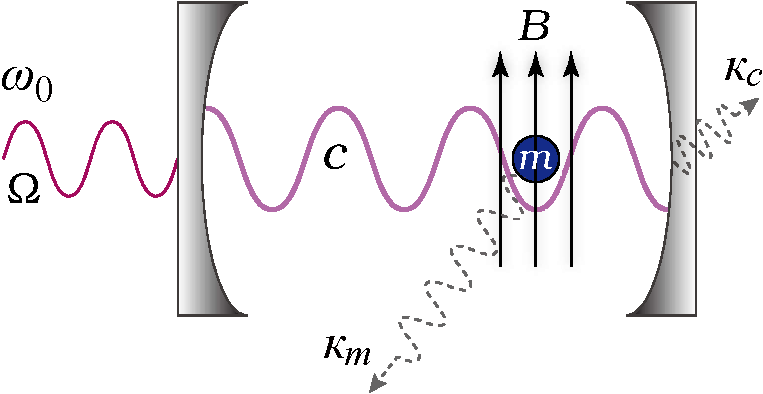
\includegraphics[width=0.5\textwidth,clip]{2_1}
	\caption{腔磁振子系统示意图} 
	\label{FigSetup}
\end{figure}

\subsection{空腔光场的量子化}
我们要想探究系统中的量子特性,就必须对微波腔中的电磁场也就是光场进行二次量子化的处理。在经典场论里介质中的无源电磁场满足Maxwell方程组
\begin{equation}
\begin{aligned}
& \nabla \times \mathbf{H}=\partial \mathbf{D} / \partial t \\
& \nabla \times \mathbf{E}=-\partial \mathbf{B} / \partial t \\
& \nabla \cdot \mathbf{B}=0 \\
& \nabla \cdot \mathbf{D}=0
\end{aligned}\label{Maxwell}
\end{equation}
对于微波腔中的电场分量和磁场分量来说YIG可以看做是各向同性的介质,我们可以得到
\begin{equation}
\mathbf{B} = \mu_{0} \mu \mathbf{H}, \quad \mathbf{D} = \varepsilon_0 \varepsilon \mathbf{E}
\end{equation}
其中$\mu_{0}$,$\varepsilon_0$分别是真空中的磁导率和介电常数,$\mu$,$\varepsilon$分别是YIG的磁导率和相对介电常数。从Maxwell方程组\eqref{Maxwell}中我们可以得到库伦规范$\nabla\cdot\mathbf{A}(\mathbf{r}, t)=0$下的波动方程
\begin{equation}
\nabla^{2} \mathbf{A}=\mu_{0}\mu \varepsilon_0\varepsilon \partial^{2} \mathbf{A} / \partial t^{2} \label{WaveFunction}
\end{equation}
其中$\mathbf{A}(\mathbf{r}, t)$是电磁场的矢势并且满足
\begin{equation}
\mathbf{E}=-\partial \mathbf{A}(\mathbf{r}, t) / \partial t, \quad \mathbf{B}=\nabla \times \mathbf{A}(\mathbf{r}, t)
\label{EBARelations}
\end{equation}

波动方程\eqref{WaveFunction}具有形式解$\mathbf{A}(\mathbf{r}, t)\propto\sum_{k} \left[A_{k} \mathbf{u}_{k}(\mathbf{r}) e^{-i \omega_{k} t}+ A_{k}^* \mathbf{u}_{k}^*(\mathbf{r}) e^{i \omega_{k} t}\right]$,二次量子化的操作就是将复振幅$A_{k}$,$A_{k}^*$替换为湮灭产生算符$c_{k}$,$c_{k}^{\dag}$:
\begin{equation}
\hat{\mathbf{A}}(\mathbf{r}, t)\propto\sum_{k} \left[c_{k} \mathbf{u}_{k}(\mathbf{r}) e^{-i \omega_{k} t}+ c_{k}^{\dag} \mathbf{u}_{k}^*(\mathbf{r}) e^{i \omega_{k} t}\right] 
\label{SecondQuantized}
\end{equation}
在这一形式下使用关系\eqref{EBARelations}计算腔中光场的能量$E_c=1/2 \int_{V}\left(\varepsilon \mathbf{E} \cdot \mathbf{E}+1/\mu \mathbf{B} \cdot \mathbf{B}\right) d V$可以得到光场的哈密顿量
\begin{equation}
\hat{H}_{\mathrm{c}} = \hbar \sum_{k} \omega_{k} c_{k}^{\dag} c_{k}
\label{CavityHamiltonian}
\end{equation}
其中$\omega_{k}$表示模式数为$k$的微波腔共振频率,在这个过程中我们需要用下面的亥姆霍兹方程定出\eqref{SecondQuantized}中的归一化系数
\begin{equation}
\left(\nabla^{2}+k^{2}\right) \mathbf{u}_{k}(\mathbf{r})=0
\label{Helmholtz}
\end{equation}
二维矢量$\mathbf{u}_{k}$表示偏振方向并且满足$\int_{V} \mathbf{u}_{k} \cdot \mathbf{u}_{k^{\prime}}^{*} \mathrm{~d}^{3} r=V \delta_{k, k^{\prime}}$,$V$表示腔的内部体积。亥姆霍兹方程\eqref{Helmholtz}还需要满足周期性边界条件,这取决于具体腔的几何外形和材质。最终定出系数的场算符写作
\begin{align}
&\hat{\mathbf{A}}(\mathbf{r}, t)= \sum_{k} \sqrt{\frac{\hbar}{2 V \varepsilon_{0} \varepsilon \omega_{k}}} \left[ c_{k} \mathbf{u}_{k}(\mathbf{r}) e^{-i \omega_{k} t} + c_{k}^{\dag} \mathbf{u}_{k}^{*} (\mathbf{r}) e^{i \omega_{k} t} \right] \\
&\hat{\mathbf{E}}(\mathbf{r}, t)=i \sum_{k} \sqrt{\frac{\hbar \omega_{k}}{2 V \varepsilon_{0} \varepsilon}} \left[ c_{k} \mathbf{u}_{k}(\mathbf{r}) e^{-i \omega_{k} t} - c_{k}^{\dag} \mathbf{u}_{k}^{*} (\mathbf{r}) e^{i \omega_{k} t} \right] \\
&\hat{\mathbf{B}}(\mathbf{r}, t)=i \sum_{k} \sqrt{\frac{\hbar}{2 V \varepsilon_{0} \varepsilon \omega_{k}}} \left[ c_{k} \mathbf{k} \times \mathbf{u}_{k}(\mathbf{r}) e^{-i \omega_{k} t} - c_{k}^{\dag} \mathbf{k}^* \times \mathbf{u}_{k}(\mathbf{r})^* e^{i \omega_{k} t} \right]
\label{BOperator}
\end{align}

\subsection{自旋波的量子化及与光场的耦合}
处于YIG球中的自旋粒子之间有着强关联相互作用,这使得它们的集体运动表现出自旋波的行为,类似于声波可以量子化为声子那样,自旋波的量子化激子被称作磁振子。自旋波的激发会引起宏观上磁性材料磁化强度的变化,我们可以从磁化强度满足的演化方程出发,使用与上一小节类似的方法也可以将YIG球中的自旋波(磁化强度)量子化。

对于在外加偏置磁场$\mathbf{H}_0$中磁化的YIG球,用$\mathbf{M}$表示它的磁化强度,此时材料的自由能可以表示为
\begin{equation}
\begin{aligned}
E=\int_{V} \mathrm{~d}^{3} r \left[\frac{A}{M_{\mathrm{s}}^{2}} \sum_{i=x, y, z}\left|\nabla M_{i}\right|^{2}+U_{\mathrm{an}}[\mathbf{M}]-\mu_{0} \mathbf{M} \cdot \mathbf{H}_{0}-\frac{\mu_{0}}{2} \mathbf{M} \cdot \mathbf{H}_{\mathrm{d}}[\mathbf{M}]\right]
\label{FreeEnergy}
\end{aligned}
\end{equation}
上式中第一项的积分表示磁化体系的交换能。第二项的积分表示各向异性能,对于常见的易轴各向异性会有正比于$M_z^2$的形式。第三项的积分表示与外加磁场间产生的Zeeman能。最后一项的积分表示退磁自能。从单个自旋的角动量定理可以得到磁化强度在无耗散时的演化方程
\begin{equation}
\dot{\mathbf{M}}=-\gamma \mathbf{M} \times \mu_{0} \mathbf{H}_{0}
\label{NoDissLLEquation}
\end{equation}
其中$\gamma=g_{\mathrm{Z}} \mu_{\mathrm{B}} / \hbar$表示旋磁比,$g_{\mathrm{Z}}$表示玻尔磁子,$\mu_{\mathrm{B}}$是电子的朗德因子。由于YIG的矫顽力很小,很容易达到饱和磁化状态,此时方程\eqref{NoDissLLEquation}的解可以理解为磁化强度在外加磁场限定的方向附近做微小震荡,即$\mathbf{M}(\mathbf{r},t)=\mathbf{M}_{\mathrm{s}}(\mathbf{r})+\delta \mathbf{M}(\mathbf{r}, t)$。我们此时所做的量子化操作如下
\begin{equation}
\delta \hat{\mathbf{M}}(\mathbf{r}, t) \propto \frac{M_{\mathrm{s}}}{2} \sum_{\eta}\left[\mathbf{w}_{\eta}(\mathbf{r}) {m}_{\eta}+\mathbf{w}_{\eta}^{*}(\mathbf{r}) {m}_{\eta}^{\dagger}\right]
\label{MOperator}
\end{equation}
其中${m}_{\eta}$,${m}_{\eta}^{\dagger}$分别表示磁振子模式$\eta$下的湮灭和产生算符,$mathbf{w}_{\eta}$是对应的无量纲振幅。同样地用这一形式计算\eqref{FreeEnergy},我们关注的是分平衡量$\delta \hat{\mathbf{M}}$产生的能量,积分项中只会包含$\delta \hat{\mathbf{M}}$的一次和二次项,而一次项的积分我们认为是零,剩下的二次项可以整理为磁振子的哈密顿量
\begin{equation}
\hat{H}_{\mathrm{m}}=\hbar \sum_{\eta} \omega_{\eta} {m}_{\eta}^{\dagger} {m}_{\eta}
\end{equation}
其中$\omega_{\eta}$表示模式${\eta}$磁振子的铁磁共振频率。磁化强度算符归一化系数的计算依赖于不同的各向异性考量,具体可以查看参考文献。

现在我们可以来考虑把YIG放置到微波腔中,并且外加偏置磁场使其饱和磁化。此时整个系统能量为
\begin{equation}
\hat{\mathcal{H}}=\int_V \left(\frac{\varepsilon}{2} \hat{\mathbf{E}}^{2}+\frac{1}{2 \mu} \hat{\mathbf{B}}^{2}-\hat{\mathbf{M}} \cdot \hat{\mathbf{B}}+\hat{\mathcal{H}}_{\mathrm{m}}\right) d \mathbf{r}
\end{equation}
可以看出上式中前两项和最后一项分别表示微波腔中光场和磁振子本身的能量密度,第三项表示磁振子与微波的磁场分量相互作用的Zeeman能。我们将场算符\eqref{BOperator}和\eqref{MOperator}代入其中就能得到腔中光与磁振子相互作用的哈密顿量
\begin{equation}
\hat{H}_{\mathrm{cm}}=\hbar \sum_{k \eta}\left(g_{k \eta} \hat{a}_{k} \hat{m}_{\eta}^{\dagger}+g_{k \eta}^{*} \hat{a}_{k}^{\dagger} \hat{m}_{\eta}\right)
\end{equation}
上式中我们已经通过旋转波近似拿掉了粒子数不守衡的项,耦合率$g_{k \eta}$为
\begin{equation}
\hbar g_{k \eta}=-\frac{M_{s}}{2} \sqrt{\frac{\hbar}{2 V \varepsilon_{0} \varepsilon \omega_{k}}} \int d \mathbf{r}\left[\nabla \times \mathbf{u}_{k}(\mathbf{r})\right] \cdot \mathbf{w}_{\eta}^{*}(\mathbf{r})
\end{equation}
不失一般性地,我们可以认为耦合率$g_{k \eta}$是实数。至此,我们得到的腔磁振子系统的总哈密顿量为
\begin{equation}
\begin{aligned}
\hat{H}_{tot}=\hat{H}_{\mathrm{c}}+\hat{H}_{\mathrm{m}}+\hat{H}_{\mathrm{cm}}
\end{aligned}
\end{equation}
由于我们考虑的微波腔一直在被外部光源驱动,所以还需要在哈密顿量中加入持续产生相干光子的驱动项
\begin{equation}
\hat{H}_{\mathrm{D}}=\sum_{p} \hbar \Omega_{p}\left({a}_{p} e^{i \omega_{\mathrm{0}} t}+{a}_{p}^{\dagger} e^{-i \omega_{\mathrm{0}} t}\right)
\end{equation}
其中$\Omega_{p}$是与光源功率$P$有关的参数,一般来说$|\Omega_{p}|^2 \propto P$。在我们的研究中主要考虑的是磁振子的基模即Kittel模与一个腔模的耦合,所使用的完整哈密顿量如下
\begin{equation}
H = \hbar\omega_{c}c^{\dag}c+\hbar\omega_{m}m^{\dag}m+\hbar gc^{\dag}m+\hbar gm^{\dag}c+i\hbar\Omega(c^{\dag}e^{-i\omega_{0}t}-ce^{i\omega_{0}t})
\label{Hamiltonian}
\end{equation}
其中$\omega_{c}$,$\omega_{m}$分别表示单个腔模和磁振子模的频率,$g$表示它们之间的耦合率。YIG球中Kittel模频率与偏置磁场满足关系$\omega_{m}=\gamma\mu_{0} \mathbf{H}_{0}=\gamma B$。

\section{主方程}
\label{secMaster}
上一节中得到的腔磁振子系统的哈密顿量\eqref{Hamiltonian}只是一个理想化的封闭模型,实际中由于需要对腔中光场进行不断的驱动与测量,系统会不可避免地受到外部环境的影响。通常来说,外部环境会转移或是吸收内部系统的能量,从而导致系统的耗散以及退相干。在量子力学中有多种方法可以用来处理这样的开放量子系统,但是由于我们想了解腔磁振子系统中量子态的具体特点,必须要使用既能描述纯态又能描述混态的密度算符,这样一来合适的方法就是这一节所要论述的主方程。

\subsection{Liouville--von Neumann方程的解}
为了在模型中加入环境的影响,我们可以假设系统$S$和外部环境$R$的耦合具有如下形式的哈密顿量:
\begin{equation}
\mathcal{H}=H_{S}+H_{R}+H_{S R}
\label{Hsr}
\end{equation}
这里$H_{S}$和$H_{R}$分别是系统和环境的哈密顿量,$H_{SR}$为相互作用的哈密顿量。我们可以先不拘泥于环境哈密顿量的具体形式,只需要知道他可以表示为温度和能量的函数。我们的目标是在无需关注环境具体状态的情形下研究混合体系$S \otimes R$中目标系统$S$的演化。为了做到这一点,需要用到密度算符的工具。我们用$\chi(t)$表示$S \otimes R$的密度算符并对环境的部分求迹,定义约化密度算符为
\begin{equation}
\rho(t) \equiv \operatorname{tr}_{R}[\chi(t)]
\end{equation}
显然,如果我们有了约化密度算符$\rho(t)$,很容易就能算出系统$S$的Hilbert空间中任一算符$\hat{O}$的平均,而不需要知道$\chi(t)$的具体形式:
\begin{equation}
\langle\hat{O}\rangle=\operatorname{tr}_{S \otimes R}[\hat{O} \chi(t)]=\operatorname{tr}_{S}\left\{\hat{O} \operatorname{tr}_{R}[\chi(t)]\right\}=\operatorname{tr}_{S}[\hat{O} \rho(t)]
\end{equation}
接下来我们要做的是得到$\rho(t)$演化方程。

%Schr\"{o}dinger
已知$\chi$的Liouville--von Neumann方程为
\begin{equation}
\dot{\chi}=\frac{1}{i \hbar}[\mathcal{H}, \chi]
\label{LMEq1}
\end{equation}
这里可以把$\mathcal{H}$中的$H_{S}+H_{R}$看作主要部分,$H_{SR}$当成次要部分,转入相互作用绘景下来方便我们的处理:
\begin{equation}
\tilde{\chi}(t) \equiv e^{(i / \hbar)\left(H_{S}+H_{R}\right) t} \chi(t) e^{-(i / \hbar)\left(H_{S}+H_{R}\right) t}
\end{equation}
结合\eqref{Hsr}、\eqref{LMEq1}与上式后可以得到
\begin{align}
\dot{\tilde{\chi}} &=\frac{i}{\hbar}\left(H_{S}+H_{R}\right) \tilde{\chi}-\frac{i}{\hbar} \tilde{\chi}\left(H_{S}+H_{R}\right)+e^{(i / \hbar)\left(H_{S}+H_{R}\right) t} \dot{\chi} e^{-(i / \hbar)\left(H_{S}+H_{R}\right) t} \notag \\
&=\frac{1}{i \hbar}\left[\tilde{H}_{S R}(t), \tilde{\chi}\right]
\label{LMEq2}
\end{align}
% oOSRHH{\ttfamily oOSRHH}{\sffamily oOSRHH}
其中$\tilde{H}_{S R}(t)$是显含时间的量:
\begin{equation}
\tilde{H}_{S R}(t) \equiv e^{(i / \hbar)\left(H_{S}+H_{R}\right) t} H_{S R} e^{-(i / \hbar)\left(H_{S}+H_{R}\right) t}
\end{equation}
对方程\eqref{LMEq2}直接积分可以得到
\begin{equation}
\tilde{\chi}(t)=\chi(0)+\frac{1}{i \hbar} \int_{0}^{t} d t^{\prime}\left[\tilde{H}_{S R}\left(t^{\prime}\right), \tilde{\chi}\left(t^{\prime}\right)\right]
\end{equation}
把上式回代到方程\eqref{LMEq2}的等号右侧:
\begin{equation}
\dot{\tilde{\chi}}=\frac{1}{i \hbar}\left[\tilde{H}_{S R}(t), \chi(0)\right]-\frac{1}{\hbar^{2}} \int_{0}^{t} d t^{\prime}\left[\tilde{H}_{S R}(t),\left[\tilde{H}_{S R}\left(t^{\prime}\right), \tilde{\chi}\left(t^{\prime}\right)\right]\right]
\label{LMExpd2}
\end{equation}
以上的推导都是严格的,我们甚至可以重复\eqref{LMEq2}到\eqref{LMExpd2}的过程来得到无限多的积分项,但是这里做到二阶就足够引入我们下面的近似了。

\subsection{Born--Markov近似}
假设$t=0$时的系统$S$和环境$R$之间没有关联但是相互作用已然存在,我们可以把$\chi(0)=\tilde{\chi}(0)$表示为
\begin{equation}
\chi(0)=\rho(0) R_{0}
\end{equation}
其中$R_{0}$是初始时刻环境的密度矩阵。记$\tilde{\chi}(t)$求迹后的密度矩阵为$\tilde{\rho}(t)$:
\begin{equation}
\operatorname{tr}_{R}[\tilde{\chi}(t)]=e^{(i / \hbar) H_{S} t} \rho(t) e^{-(i / \hbar) H_{S} t} \equiv \tilde{\rho}(t)
\label{InitialAssumption}
\end{equation}
对方程\eqref{LMExpd2}进行求迹运算后我们就可以得到如下的主方程:
\begin{equation}
\dot{\tilde{\rho}}=-\frac{1}{\hbar^{2}} \int_{0}^{t} d t^{\prime} \operatorname{tr}_{R}\left\{\left[\tilde{H}_{S R}(t),\left[\tilde{H}_{S R}\left(t^{\prime}\right), \tilde{\chi}\left(t^{\prime}\right)\right]\right]\right\}
\label{MasterEq}
\end{equation}
这里我们已经通过假设$\operatorname{tr}_{R}\left[\tilde{H}_{S R}(t) R_{0}\right]=0$消去了\eqref{LMExpd2}中的第一项。这项假设需要相互作用$H_{S R}$在$R_{0}$态下的平均值为零,我们总是可以满足这个条件,只用在哈密顿量里考虑是否加入$\operatorname{tr}_{R}\left(H_{S R} R_{0}\right)$即可。

虽然已经假设了初始时$S$和$R$无关,但由于相互作用的存在,之后的时刻里必然会出现新的关联,我们需要在这里引入Born近似。Born近似要求系统和环境间的相互作用是微弱的,这样一来系统就几乎不会对环境有反作用的影响。在这一近似下,环境的状态不随时间改变并且在相互作用中也一直保持不变。此外,Born近似也意味着在处理$\chi(t)$受到的环境影响时只包含$H_{SR}$的同阶量。这样一来,我们就可以把$\tilde{\chi}(t)$写作
\begin{equation}
\tilde{\chi}(t)=\tilde{\rho}(t) R_{0}+O\left(H_{S R}\right)
\end{equation}
这也可以等价的表述为:系统与环境的整体态$\tilde{\chi}(t)$的未来仅由系统态$\tilde{\rho}(t)$决定,而不依赖于环境态的历史。把Born近似应用于方程\eqref{MasterEq}并忽略掉$H_{S R}$的高阶项可以得到
\begin{equation}
\dot{\tilde{\rho}}=-\frac{1}{\hbar^{2}} \int_{0}^{t} d t^{\prime} \operatorname{tr}_{R}\left\{\left[\tilde{H}_{S R}(t),\left[\tilde{H}_{S R}\left(t^{\prime}\right), \tilde{\rho}\left(t^{\prime}\right) R_{0}\right]\right]\right\}
\label{MasterEqBorn}
\end{equation}

仔细观察上面的方程,我们会发现$\tilde{\rho}(t)$依赖于它自身的历史$\tilde{\rho}\left(t^{\prime}\right)$。换句话说,方程\eqref{MasterEqBorn}并不是Markov型的。Markov型的系统要求它的未来只取决于它现在的状态。所以我们另一个要做的主要近似就是把$\tilde{\rho}\left(t^{\prime}\right)$替换为$\tilde{\rho}(t)$,这样我们就得到了Born--Markov近似下的主方程:
\begin{equation}
\dot{\tilde{\rho}}=-\frac{1}{\hbar^{2}} \int_{0}^{t} d t^{\prime} \operatorname{tr}_{R}\left\{\left[\tilde{H}_{S R}(t),\left[\tilde{H}_{S R}\left(t^{\prime}\right), \tilde{\rho}(t) R_{0}\right]\right]\right\}
\end{equation}
Markov近似在物理上是合理的。具体来讲,系统$S$之所以依赖于它的历史是因为通过相互作用$H_{SR}$系统的早期态会映照在改变后的环境态上,而随后的早期态又会被改变后的环境态经过相互作用映照下来。但如果环境是一个一直处于热平衡的庞大系统,也就是热库的话,它就不会保持住来自$S$的改变太长时间。这样一来关键就在于比较热库的关联时间与系统$S$能发生明显变化的时间相比是否远远地小。下面来验证一下上述说法。

我们给定相互作用$H_{SR}$一个具体点的形式
\begin{equation}
H_{S R}=\hbar \sum_{i} s_{i} \Gamma_{i}
\label{HsrSpec}
\end{equation}
这里的$s_{i}$是系统$S$的Hilbert空间里的算符,$\Gamma_{i}$是热库$R$的Hilbert空间里的算符。然后依照上一节所述在相互作用表象下有
\begin{equation}
\begin{aligned}
\tilde{H}_{S R}(t) &=\hbar \sum_{i} e^{(i / \hbar)\left(H_{S}+H_{R}\right) t} s_{i} \Gamma_{i} e^{-(i / \hbar)\left(H_{S}+H_{R}\right) t} \\
&=\hbar \sum_{i}\left(e^{(i / \hbar) H_{S} t} s_{i} e^{-(i / \hbar) H_{S} t}\right)\left(e^{(i / \hbar) H_{R} t} \Gamma_{i} e^{-(i / \hbar) H_{R} t}\right) \\
&=\hbar \sum_{i} \tilde{s}_{i}(t) \tilde{\Gamma}_{i}(t)
\label{HsrSpec2}
\end{aligned}
\end{equation}
此时Born近似的主方程\eqref{MasterEqBorn}就变为了
\begin{align}
\dot{\tilde{\rho}}=&-\sum_{i, j} \int_{0}^{t} d t^{\prime} \operatorname{tr}_{R}\left\{\left[\tilde{s}_{i}(t) \tilde{\Gamma}_{i}(t),\left[\tilde{s}_{j}\left(t^{\prime}\right) \tilde{\Gamma}_{j}\left(t^{\prime}\right), \tilde{\rho}\left(t^{\prime}\right) R_{0}\right]\right]\right\} \notag \\
=&-\sum_{i, j} \int_{0}^{t} d t^{\prime}\left\{\tilde{s}_{i}(t) \tilde{s}_{j}\left(t^{\prime}\right) \tilde{\rho}\left(t^{\prime}\right) \operatorname{tr}_{R}\left[\tilde{\Gamma}_{i}(t) \tilde{\Gamma}_{j}\left(t^{\prime}\right) R_{0}\right]\right. \notag \\
&-\tilde{s}_{i}(t) \tilde{\rho}\left(t^{\prime}\right) \tilde{s}_{j}\left(t^{\prime}\right) \operatorname{tr}_{R}\left[\tilde{\Gamma}_{i}(t) R_{0} \tilde{\Gamma}_{j}\left(t^{\prime}\right)\right]-\tilde{s}_{j}\left(t^{\prime}\right) \tilde{\rho}\left(t^{\prime}\right) \tilde{s}_{i}(t) \notag \\
&\left.\times \operatorname{tr}_{R}\left[\tilde{\Gamma}_{j}\left(t^{\prime}\right) R_{0} \tilde{\Gamma}_{i}(t)\right]+\tilde{\rho}\left(t^{\prime}\right) \tilde{s}_{j}\left(t^{\prime}\right) \tilde{s}_{i}(t) \operatorname{tr}_{R}\left[R_{0} \tilde{\Gamma}_{j}\left(t^{\prime}\right) \tilde{\Gamma}_{i}(t)\right]\right\} \notag \\
=&-\sum_{i, j} \int_{0}^{t} d t^{\prime}\left\{\left[\tilde{s}_{i}(t) \tilde{s}_{j}\left(t^{\prime}\right) \tilde{\rho}\left(t^{\prime}\right)-\tilde{s}_{j}\left(t^{\prime}\right) \tilde{\rho}\left(t^{\prime}\right) \tilde{s}_{i}(t)\right]\left\langle\tilde{\Gamma}_{i}(t) \tilde{\Gamma}_{j}\left(t^{\prime}\right)\right\rangle_{R}\right. \label{MasterEqBorn2} \\
&\left.+\left[\tilde{\rho}\left(t^{\prime}\right) \tilde{s}_{j}\left(t^{\prime}\right) \tilde{s}_{i}(t)-\tilde{s}_{i}(t) \tilde{\rho}\left(t^{\prime}\right) \tilde{s}_{j}\left(t^{\prime}\right)\right]\left\langle\tilde{\Gamma}_{j}\left(t^{\prime}\right) \tilde{\Gamma}_{i}(t)\right\rangle_{R}\right\} \notag 
\end{align}
在上式的推导中我们用到了求迹运算的循环特性---$\operatorname{tr}\left( \hat{A} \hat{B} \hat{C} \right)=\operatorname{tr}\left(\hat{C} \hat{A} \hat{B} \right)= \operatorname{tr} \left( \hat{B} \hat{C} \hat{A} \right)$以及简化符号
\begin{equation}
\begin{aligned}
\left\langle\tilde{\Gamma}_{i}(t) \tilde{\Gamma}_{j}\left(t^{\prime}\right)\right\rangle_{R} &=\operatorname{tr}_{R}\left[R_{0} \tilde{\Gamma}_{i}(t) \tilde{\Gamma}_{j}\left(t^{\prime}\right)\right] \\
\left\langle\tilde{\Gamma}_{j}\left(t^{\prime}\right) \tilde{\Gamma}_{i}(t)\right\rangle_{R} &=\operatorname{tr}_{R}\left[R_{0} \tilde{\Gamma}_{j}\left(t^{\prime}\right) \tilde{\Gamma}_{i}(t)\right]
\end{aligned}
\end{equation}
热库的影响在方程\eqref{MasterEqBorn2}中体现为上式的两个关联函数。我们认为关联函数的变化在时间尺度上远快于$\tilde{\rho}(t)$的变化,理想情况下可以取
\begin{equation}
\left\langle\tilde{\Gamma}_{i}(t) \tilde{\Gamma}_{j}\left(t^{\prime}\right)\right\rangle_{R} \propto \delta\left(t-t^{\prime}\right)
\end{equation}
容易看出这样做的效果就等同于我们把$\tilde{\rho}(t^{\prime})$替换为$\tilde{\rho}(t)$。

\subsection{腔磁振子系统的主方程}
我们回到腔磁振子系统的哈密顿量\eqref{Hamiltonian},把热环境看作包含各种频率的谐振子的集合,并且认为系统内的光场和磁振子各自耦合于独立的热库
\begin{equation}
\begin{aligned}
H_S\equiv{}&\hbar\omega_{c}c^{\dag}c+\hbar\omega_{m}m^{\dag}m+\hbar gc^{\dag}m+\hbar gm^{\dag}c \\
&+i\hbar\Omega(c^{\dag}e^{-i\omega_{0}t}-ce^{i\omega_{0}t}) \\
H_{R}\equiv&\sum_{i}\hbar\omega_{i}a_{i}^{\dag}a_{i}+\sum_{j}\hbar\omega_{j}b_{j}^{\dag}b_{j} \\
H_{SR}\equiv&\sum_{i}g_{c,i}(c^{\dag}a_{i}+a_{i}^{\dag}c)+\sum_{j}g_{m,j}(m^{\dag}b_{j}+b_{j}^{\dag}m)
\label{HamCMRes}
\end{aligned}
\end{equation}
其中$a(a^{\dag})$,$b(b^{\dag})$分别为光子和谐振子热库的湮灭(产生)算符,$\omega_{i}$,$\omega_{j}$表示它们的频率,光子和谐振子与热库的耦合率分别为$g_{c,i}$,$g_{m,j}$。假设热库处于热平衡的温度为$T$,则其密度算符表示为
\begin{equation}
R_{0}=\prod_{i} e^{-\hbar \omega_{i} a_{i}^{\dag}a_{i} / k_{B} T}\left(1-e^{-\hbar \omega_{i} / k_{B} T}\right) \otimes \prod_{j} e^{-\hbar \omega_{j} b_{j}^{\dag}b_{j} / k_{B} T}\left(1-e^{-\hbar \omega_{j} / k_{B} T}\right)
\label{ThermalState}
\end{equation}
其中$k_{B}$表示玻尔兹曼常数,$R_{0}$即为满足玻色--爱因斯坦分布的密度算符。值得注意的是,关于\eqref{HamCMRes}中的$H_{SR}$,这里已经通过旋转波近似略去了粒子数不守衡的项,但是对于有着超强耦合的系统这一近似就不再成立,具体的讨论见相关研究\cite{PhysRevA.98.053834Ridolfo}。

把哈密顿量\eqref{HamCMRes}对照上一小节\eqref{HsrSpec}的形式表示为
\begin{equation}
\begin{gathered}
s_{1}=c, \quad s_{2}=c^{\dagger}, \quad s_{3}=m, \quad s_{4}=m^{\dagger} \\
\Gamma_{1}= \sum_{i} g_{c,i} a_{i}^{\dag}, \quad \Gamma_{2}= \sum_{i} g_{c,i} a_{i}, \quad \Gamma_{3}= \sum_{j} g_{m,j} b_{j}^{\dag}, \quad \Gamma_{4}= \sum_{j} g_{m,j} b_{j}
\end{gathered}
\end{equation}
然后\eqref{HsrSpec2}中的算符就变为了
\begin{equation}
\begin{aligned}
&\tilde{s}_{1}(t)=e^{(i / \hbar) H_{S} t} c e^{-(i / \hbar) H_{S} t} \approx e^{i \omega_{c}c^{\dag}c t} e^{i \omega_{m}m^{\dag}m t} c e^{-i \omega_{c}c^{\dag}c t} e^{-i \omega_{m}m^{\dag}m t} = c e^{-i \omega_{c} t} \\
&\tilde{s}_{2}(t)=e^{(i / \hbar) H_{S} t} c^{\dagger} e^{-(i / \hbar) H_{S} t} \approx e^{i \omega_{c}c^{\dag}c t} e^{i \omega_{m}m^{\dag}m t} c^{\dagger} e^{-i \omega_{c}c^{\dag}c t} e^{-i \omega_{m}m^{\dag}m t} = c^{\dagger} e^{i \omega_{c} t} \\
&\tilde{s}_{3}(t)=e^{(i / \hbar) H_{S} t} m e^{-(i / \hbar) H_{S} t} \approx e^{i \omega_{c}c^{\dag}c t} e^{i \omega_{m}m^{\dag}m t} m e^{-i \omega_{c}c^{\dag}c t} e^{-i \omega_{m}m^{\dag}m t} = m e^{-i \omega_{m} t} \\
&\tilde{s}_{4}(t)=e^{(i / \hbar) H_{S} t} m^{\dagger} e^{-(i / \hbar) H_{S} t} \approx e^{i \omega_{c}c^{\dag}c t} e^{i \omega_{m}m^{\dag}m t} m^{\dagger} e^{-i \omega_{c}c^{\dag}c t} e^{-i \omega_{m}m^{\dag}m t} =m^{\dagger} e^{i \omega_{m} t}
\label{interactS}
\end{aligned}
\end{equation}
以及
\begin{equation}
\begin{aligned}
\tilde{\Gamma}_{1}(t) &=\exp \left(i \sum_{n}\omega_{n}a_{n}^{\dag}a_{n} t\right) \sum_{i} g_{c,i} a_{i}^{\dag} \exp \left(-i \sum_{m}\omega_{m}a_{m}^{\dag}a_{m} t\right) =\sum_{i} g_{c,i} a_{i}^{\dag} e^{i \omega_{i} t} \\
\tilde{\Gamma}_{2}(t) &=\exp \left(i \sum_{n}\omega_{n}a_{n}^{\dag}a_{n} t\right) \sum_{i} g_{c,i} a_{i} \exp \left(-i \sum_{m}\omega_{m}a_{m}^{\dag}a_{m} t\right) =\sum_{i} g_{c,i} a_{i} e^{-i \omega_{i} t} \\
\tilde{\Gamma}_{3}(t) &=\exp \left(i \sum_{n}\omega_{n}b_{n}^{\dag}b_{n} t\right) \sum_{j} g_{m,j} b_{j}^{\dag} \exp \left(-i \sum_{m}\omega_{m}b_{m}^{\dag}b_{m} t\right) =\sum_{j} g_{m,j} b_{j}^{\dag} e^{i \omega_{j} t} \\
\tilde{\Gamma}_{4}(t) &=\exp \left(i \sum_{n}\omega_{n}b_{n}^{\dag}b_{n} t\right) \sum_{j} g_{m,j} b_{j} \exp \left(-i \sum_{m}\omega_{m}b_{m}^{\dag}b_{m} t\right) =\sum_{j} g_{m,j} b_{j} e^{-i \omega_{j} t}
\label{interactGam}
\end{aligned}
\end{equation}
在\eqref{interactS}的推导中我们用到了$H_S$中耦合项与驱动项远远小于光子和谐振子谐振能量的假设,在下一章节的参数选取时我们会知道这在实验上是合理的,而在\eqref{interactGam}的推导中我们则用到了不同模式谐振子算符相互对易的特点。另外还需要注意的是,结合\eqref{ThermalState}与\eqref{interactGam}可以得到$\left\langle\tilde{\Gamma}_{1}(t)\right\rangle_{R_0}=\left\langle\tilde{\Gamma}_{2}(t)\right\rangle_{R_0}=\left\langle\tilde{\Gamma}_{3}(t)\right\rangle_{R_0}=\left\langle\tilde{\Gamma}_{4}(t)\right\rangle_{R_0}=0$,也就是说式\eqref{InitialAssumption}的假设是成立的。

现在让我们来继续推导方程\eqref{MasterEqBorn2},由于求和指标需要遍历$i=1,2,3,4$以及$j=1,2,3,4$,故需要计算64项的积分值,好在其中一半以上的项都是能拿掉的,容易计算出
\begin{align}
	\left\langle\tilde{\Gamma}_{1}(t) \tilde{\Gamma}_{3}\left(t^{\prime}\right)\right\rangle_{R_0} &=\left\langle\tilde{\Gamma}_{1}(t) \tilde{\Gamma}_{4}\left(t^{\prime}\right)\right\rangle_{R_0}=\left\langle\tilde{\Gamma}_{2}(t) \tilde{\Gamma}_{3}\left(t^{\prime}\right)\right\rangle_{R_0}=\left\langle\tilde{\Gamma}_{2}(t) \tilde{\Gamma}_{4}\left(t^{\prime}\right)\right\rangle_{R_0}=0 
	\label{zeroCorrelations} \\
	\left\langle\tilde{\Gamma}_{3}(t) \tilde{\Gamma}_{1}\left(t^{\prime}\right)\right\rangle_{R_0} &=\left\langle\tilde{\Gamma}_{4}(t) \tilde{\Gamma}_{1}\left(t^{\prime}\right)\right\rangle_{R_0}=\left\langle\tilde{\Gamma}_{3}(t) \tilde{\Gamma}_{2}\left(t^{\prime}\right)\right\rangle_{R_0}=\left\langle\tilde{\Gamma}_{4}(t) \tilde{\Gamma}_{2}\left(t^{\prime}\right)\right\rangle_{R_0}=0
\end{align}
以及
\begin{equation}
\left\langle\tilde{\Gamma}_{1}(t) \tilde{\Gamma}_{1}\left(t^{\prime}\right)\right\rangle_{R_0} =\left\langle\tilde{\Gamma}_{2}(t) \tilde{\Gamma}_{2}\left(t^{\prime}\right)\right\rangle_{R_0}=\left\langle\tilde{\Gamma}_{3}(t) \tilde{\Gamma}_{3}\left(t^{\prime}\right)\right\rangle_{R_0}=\left\langle\tilde{\Gamma}_{4}(t) \tilde{\Gamma}_{4}\left(t^{\prime}\right)\right\rangle_{R_0}=0
\label{zeroCorrelations2}
\end{equation}
上面的关联函数\eqref{zeroCorrelations}--\eqref{zeroCorrelations2}以及其厄米共轭的值都是零,这样就大大简化了方程的形式,余下不为零的关联函数为
\begin{align}
\left\langle\tilde{\Gamma}_{1}(t) \tilde{\Gamma}_{2}\left(t^{\prime}\right)\right\rangle_{R_0} &=\sum_{i, k} g_{c,i} g_{c,k} e^{i \omega_{i} t} e^{-i \omega_{k} t^{\prime}} \operatorname{tr}_{R}\left(R_{0} a_{i}^{\dag} a_{k}\right) \notag \\
&=\sum_{i} g_{c,i}^{2} e^{i \omega_{i}\left(t-t^{\prime}\right)} \overline{n}_c\left(\omega_{i}, T\right) \label{Correlations1}
\end{align}
\begin{align}
\left\langle\tilde{\Gamma}_{2}(t) \tilde{\Gamma}_{1}\left(t^{\prime}\right)\right\rangle_{R_0} &=\sum_{i, k} g_{c,i} g_{c,k} e^{-i \omega_{i} t} e^{i \omega_{k} t^{\prime}} \operatorname{tr}_{R}\left(R_{0} a_{i} a_{k}^{\dag}\right) \notag \\
&=\sum_{i} g_{c,i}^{2} e^{-i \omega_{i}\left(t-t^{\prime}\right)} \left[\overline{n}_c \left(\omega_{i}, T\right)+1\right]
\end{align}
\begin{align}
\left\langle\tilde{\Gamma}_{3}(t) \tilde{\Gamma}_{4}\left(t^{\prime}\right)\right\rangle_{R_0} &=\sum_{j, k} g_{m,j} g_{m,k} e^{i \omega_{j} t} e^{-i \omega_{k} t^{\prime}} \operatorname{tr}_{R}\left(R_{0} b_{j}^{\dagger} b_{k}\right) \notag \\
&=\sum_{j} g_{m,j}^{2} e^{i \omega_{j}\left(t-t^{\prime}\right)} \overline{n}_m\left(\omega_{j}, T\right)
\end{align}
\begin{align}
\left\langle\tilde{\Gamma}_{4}(t) \tilde{\Gamma}_{3}\left(t^{\prime}\right)\right\rangle_{R_0} &=\sum_{j, k} g_{m,j} g_{m,k} e^{-i \omega_{j} t} e^{i \omega_{k} t^{\prime}} \operatorname{tr}_{R}\left(R_{0} b_{j} b_{k}^{\dagger}\right) \notag \\
&=\sum_{j} g_{m,j}^{2} e^{-i \omega_{j}\left(t-t^{\prime}\right)}\left[\overline{n}_m\left(\omega_{j}, T\right)+1\right] \label{Correlations4}
\end{align}
其中
\begin{equation}
\begin{aligned}
\overline{n}_c\left(\omega_{i}, T\right) &=\operatorname{tr}_{R}\left(R_{0} a_{i}^{\dagger} a_{i}\right)=\frac{e^{-\hbar \omega_{i} / k_{B} T}}{1-e^{-\hbar \omega_{i} / k_{B} T}}
\\
\overline{n}_m\left(\omega_{j}, T\right) &=\operatorname{tr}_{R}\left(R_{0} b_{j}^{\dagger} b_{j}\right)=\frac{e^{-\hbar \omega_{j} / k_{B} T}}{1-e^{-\hbar \omega_{j} / k_{B} T}}
\end{aligned}
\end{equation}
分别为热平衡下光子和磁振子对应温度$T$与模式$\omega_{i}$,$\omega_{j}$下的平均光子数和磁振子数。

非零关联函数\eqref{Correlations1}--\eqref{Correlations4}中需要对所有模式的热库求和,我们用$G_{a(b)}(\omega)$表示光子(磁振子)所处热库的态密度,$G_{a(b)}(\omega) d\omega$表示$\omega$到$\omega+d\omega$频率间隔内的光子(磁振子)数,这样就可以将求和变为积分。在做了变量替换$\tau = t-t^{\prime}$后,Born近似的主方程可以化简为
\begin{equation}
\begin{aligned}
\dot{\tilde{\rho}}={}&-\int_{0}^{t} d \tau \biggl\{\left[c c^{\dagger} \tilde{\rho}(t-\tau)-c^{\dagger} \tilde{\rho}(t-\tau) c\right] e^{-i \omega_{c} \tau}\left\langle\tilde{\Gamma}_1(t) \tilde{\Gamma}_2(t-\tau)\right\rangle_{R_0}+\text { h.c. }\\
&+\left[c^{\dagger} c \tilde{\rho}(t-\tau)-c \tilde{\rho}(t-\tau) c^{\dagger}\right] e^{i \omega_{c} \tau}\left\langle\tilde{\Gamma}_2(t) \tilde{\Gamma}_1(t-\tau)\right\rangle_{R_0}+\text { h.c. } \\
&+\left[m m^{\dagger} \tilde{\rho}(t-\tau)-m^{\dagger} \tilde{\rho}(t-\tau) m\right] e^{-i \omega_{m} \tau}\left\langle\tilde{\Gamma}_3(t) \tilde{\Gamma}_4(t-\tau)\right\rangle_{R_0}+\text { h.c. }\\
&+\left[m^{\dagger} m \tilde{\rho}(t-\tau)-m \tilde{\rho}(t-\tau) m^{\dagger}\right] e^{i \omega_{m} \tau}\left\langle\tilde{\Gamma}_4(t) \tilde{\Gamma}_3(t-\tau)\right\rangle_{R_0}+\text { h.c. } \biggr\}
\label{MasterEqBorn3}
\end{aligned}
\end{equation}
%书中的方程倒数第二项算符的顺序无误
关联函数也化为了
\begin{align}
\left\langle\tilde{\Gamma}_{1}(t) \tilde{\Gamma}_{2}\left(t^{\prime}\right)\right\rangle_{R_0} &=\int_{0}^{\infty} d \omega e^{i \omega \tau} G_a(\omega) g_{c}^{2}(\omega) \overline{n}_c\left(\omega, T\right) \label{} \\
\left\langle\tilde{\Gamma}_{2}(t) \tilde{\Gamma}_{1}\left(t^{\prime}\right)\right\rangle_{R_0} &=\int_{0}^{\infty} d \omega e^{-i \omega \tau} G_a(\omega) g_{c}^{2}(\omega) \left[\overline{n}_c \left(\omega, T\right)+1\right] \\
\left\langle\tilde{\Gamma}_{3}(t) \tilde{\Gamma}_{4}\left(t^{\prime}\right)\right\rangle_{R_0} &=\int_{0}^{\infty} d \omega e^{i \omega \tau} G_b(\omega) g_{m,j}^{2} \overline{n}_m\left(\omega, T\right) \\
\left\langle\tilde{\Gamma}_{4}(t) \tilde{\Gamma}_{3}\left(t^{\prime}\right)\right\rangle_{R_0} &=\int_{0}^{\infty} d \omega e^{-i \omega \tau} G_b(\omega) g_{m,j}^{2} \left[\overline{n}_m\left(\omega, T\right)+1\right] \label{}
\end{align}
%书中这部分的推导有提到积分中的高频平均掉了低频,是因为各个量的相乘关系导致积分时低频的包络都成了0。旋转波近似中有一个高频被平均掉的说法,是因为高频和低频的相加关系。
方程\eqref{MasterEqBorn3}的积分中存在着三种时间尺度,其中热库的关联函数有着极窄的线型\cite{carmichael1999statistical},其有效关联时间$t_R \sim \hbar/k_B T \approx 10^{-12}s$。而在腔磁振子系统中,系统$\tilde{\rho} (t-\tau)$能发生明显变化的时间取决于耦合率以及关联函数,在实验参数中$t_S \sim 10^{-7}s$。振荡项$e^{-i \omega_{c(m)} \tau}$在微波频域内的时间尺度$t_0 \sim 10^{-10}s$。因此在$t_S$时间尺度内对 $\tau$ 积分时$\tilde{\rho}$可以看作是不变的,换句话说,我们可以直接将$\tilde{\rho} (t-\tau)$替换为$\tilde{\rho} (t)$,也就是使用Markov近似将$\tilde{\rho}$从积分中提出来,剩余的项可以积分为
\begin{equation}
\begin{aligned}
&\int_{0}^{t} d \tau \int_{0}^{\infty} d \omega e^{-i\left(\omega-\omega_{c}\right) \tau} G_a(\omega) g_{c}^{2}(\omega) \\
={}&\pi G_a(\omega_c) g_{c}^{2}(\omega_c)+i P \int_{0}^{\infty} d \omega \frac{G_a(\omega) g_{c}^{2}(\omega)}{\omega_{c}-\omega} \\
&\int_{0}^{t} d \tau \int_{0}^{\infty} d \omega e^{-i\left(\omega-\omega_{c}\right) \tau} G_a(\omega) g_{c}^{2}(\omega) \overline{n}_c(\omega, T) \\
={}&\pi G_a(\omega_c) g_{c}^{2}(\omega_c)\overline{n}_c(\omega_c)+i P \int_{0}^{\infty} d \omega \frac{G_a(\omega) g_{c}^{2}(\omega)}{\omega_{c}-\omega} \overline{n}_c(\omega, T) \\
&\int_{0}^{t} d \tau \int_{0}^{\infty} d \omega e^{-i\left(\omega-\omega_{m}\right) \tau} G_b(\omega) g_{m}^{2}(\omega) \\
={}&\pi G_b(\omega_m) g_{m}^{2}(\omega_m)+i P \int_{0}^{\infty} d \omega \frac{G_b(\omega) g_{m}^{2}(\omega)}{\omega_{m}-\omega} \\
&\int_{0}^{t} d \tau \int_{0}^{\infty} d \omega e^{-i\left(\omega-\omega_{m}\right) \tau} G_b(\omega) g_{m}^{2}(\omega) \overline{n}_m(\omega, T) \\
={}&\pi G_b(\omega_m) g_{m}^{2}(\omega_m)\overline{n}_m(\omega_m)+i P \int_{0}^{\infty} d \omega \frac{G_b(\omega) g_{m}^{2}(\omega)}{\omega_{m}-\omega} \overline{n}_m(\omega, T)
\label{IntergralCorrelations}
\end{aligned}
\end{equation}
上面的积分中我们用到了如下的关系式
\begin{equation}
\lim _{t \rightarrow \infty} \int_{0}^{t} d \tau e^{-i\left(\omega-\omega^{\prime}\right) \tau}=\pi \delta\left(\omega-\omega^{\prime}\right)+i \frac{P}{\omega^{\prime}-\omega}
\end{equation}
其中P表示柯西积分主值。

我们定义如下符号
\begin{align}
\Delta_c \equiv P \int_{0}^{\infty} d \omega \frac{G_a(\omega) g_{c}^{2}(\omega)}{\omega_{c}-\omega},
&\quad \Delta_m \equiv P \int_{0}^{\infty} d \omega \frac{G_b(\omega) g_{m}^{2}(\omega)}{\omega_{m}-\omega} \\
\kappa_c \equiv 2 \pi G_a\left(\omega_{c}\right)g_{c}^{2}(\omega_c),
&\quad \kappa_m \equiv 2 \pi G_b\left(\omega_{m}\right)g_{m}^{2}(\omega_m) \\
\overline{n}_c \equiv \overline{n}_c\left(\omega_{c}, T\right),\label{KcKmDefination}
&\quad \overline{n}_m \equiv \overline{n}_m\left(\omega_{m}, T\right)
\end{align}
结合\eqref{MasterEqBorn3}--\eqref{IntergralCorrelations}后,我们就得到了Born--Markov近似下腔磁振子系统的主方程
\begin{equation}
\begin{aligned}
\dot{\tilde{\rho}}={}&-i \Delta_c\left[c^{\dagger} c, \tilde{\rho}\right]+\kappa_c\left(2 c \tilde{\rho} c^{\dagger}-c^{\dagger} c \tilde{\rho}-\tilde{\rho} c^{\dagger} c\right) \\
&+2 \kappa_c \overline{n}_c\left(c \tilde{\rho} c^{\dagger}+c^{\dagger} \tilde{\rho} c-c^{\dagger} c \tilde{\rho}-\tilde{\rho} c c^{\dagger}\right) \\
&-i \Delta_m\left[m^{\dagger} m, \tilde{\rho}\right]+\kappa_m\left(2 m \tilde{\rho} m^{\dagger}-m^{\dagger} m \tilde{\rho}-\tilde{\rho} m^{\dagger} m\right) \\
&+2 \kappa_m \overline{n}_m\left(m \tilde{\rho} m^{\dagger}+m^{\dagger} \tilde{\rho} m-m^{\dagger} m \tilde{\rho}-\tilde{\rho} m m^{\dagger}\right)
\end{aligned}
\end{equation}
这里的$\tilde{\rho}$还依旧是相互作用绘景下的密度算符,通过公式\eqref{InitialAssumption}可以得到
\begin{equation}
\dot{\rho}=\frac{1}{i \hbar}\left[H_{S}, \rho\right]+e^{-(i / \hbar) H_{S} t} \dot{\tilde{\rho}} e^{(i / \hbar) H_{S} t}
\end{equation}
借助上式将$\tilde{\rho}$变换为$\rho$之后,我们就得到了所需的薛定谔绘景下的主方程
\begin{equation}
\begin{aligned}
\dot{\rho}={}&\frac{1}{i \hbar}\left[H_{S}, \rho\right]-i \Delta_c\left[c^{\dagger} c, \rho\right]-i \Delta_m\left[m^{\dagger} m, \rho\right] \\
&+\kappa_c\left(2 c \rho c^{\dagger}-c^{\dagger} c \rho-\rho c^{\dagger} c\right) \\
&+2 \kappa_c \overline{n}_c\left(c \rho c^{\dagger}+c^{\dagger} \rho c-c^{\dagger} c \rho-\rho c c^{\dagger}\right) \\
&+\kappa_m\left(2 m \rho m^{\dagger}-m^{\dagger} m \rho-\rho m^{\dagger} m\right) \\
&+2 \kappa_m \overline{n}_m\left(m \rho m^{\dagger}+m^{\dagger} \rho m-m^{\dagger} m \rho-\rho m m^{\dagger}\right)
\end{aligned}
\end{equation}
上式中的第二项与第三项的作用相当于给系统中的光子和磁振子的共振频率产生一个平移,实际上实验中不会对平移前后的频率做出区分,为了便于讨论,后面的书写中我们也不区分频移。把$\Delta_c$,$\Delta_m$归到$H_S$里,并且采用Lindblad形式书写主方程为
\begin{equation}
\dot{\rho}=\frac{1}{i\hbar}[H_S,\rho]+\mathcal{L}\{\rho\}
\label{MasterEquation}
\end{equation}
其中$\mathcal{L}$为Liouvillian超算符,定义为$\mathcal{L}\{\rho\}=\sum\limits_{o=c,m}[\kappa_{o}(1 +\overline{n}_{o})(2o\rho o^{\dag}-\{o^{\dag}o,\rho\}) +\kappa_{o} \overline{n}_{o} (2o^{\dag}\rho o-\{oo^{\dag},\rho\})]$。

\section{Fokker-Planck方程}
\label{sec3.2}
主方程\eqref{MasterEquation}是由量子力学算符构成的方程,多数情况下直接求解$\rho$会非常困难,即使是数值求解也需要选择合适的一组基来展开才能得到比较好的结果。我们这一节要做的是借助量子力学的相干态表象把这一关于算符的方程转换为关于经典复数变量的微积分方程。

\subsection{Glauber-Sudarshan $P$表象}
首先来看一下相干态$|\alpha\rangle$和$|\beta\rangle$的定义
\begin{equation}
\begin{aligned}
c|\alpha\rangle=\alpha|\alpha\rangle,& \quad\langle\alpha| c^{\dagger}=(c|\alpha\rangle)^{\dagger}=\alpha^{*}\langle\alpha| \\
m|\beta\rangle=\beta|\beta\rangle,& \quad\langle\beta| m^{\dagger}=(m|\beta\rangle)^{\dagger}=\beta^{*}\langle\beta|
\end{aligned}
\end{equation}
即相干态是湮灭算符的本征态。

由于相干态具有超完备性
\begin{equation}
\frac{1}{\pi} \int d^{2} \alpha|\alpha\rangle\langle\alpha|=1, \quad
\frac{1}{\pi} \int d^{2} \beta|\beta\rangle\langle\beta|=1
\end{equation}
所以我们可以在相干态的基下对密度算符$\rho$进行展开
\begin{equation}
\rho=\int d^{2}\alpha d^{2}\beta P(\alpha,\alpha^{*},\beta,\beta^{*},t)|\alpha,\beta\rangle \langle \alpha,\beta| \label{Pfun} 
\end{equation}
上式定义中的表象即为 Glauber-Sudarshan $P$表象,简称为$P$表象,其中的积分定义在整个复平面上,也就是$d^{2} \alpha d^{2} \beta=d(\operatorname{Re}\{\alpha\}) d(\operatorname{Im}\{\alpha\}) d(\operatorname{Re}\{\beta\}) d(\operatorname{Im}\{\beta\})$。$P$表象中的函数$P(\alpha,\alpha^{*},\beta,\beta^{*},t)$是实数,这一点由密度算符$\rho$的厄米性所保证,同时具有如下性质
\begin{equation}
\begin{aligned}
\int d^{2} \alpha d^{2}\beta P &=\int d^{2} \alpha d^{2}\beta \langle\alpha,\beta \mid \alpha,\beta \rangle P \\
&=\operatorname{tr}\left(\int d^{2} \alpha d^{2}\beta |\alpha,\beta\rangle\langle\alpha,\beta| P\right) \\
&=\operatorname{tr}(\rho) \\
&=1
\end{aligned}
\end{equation}
由此我们说$P$函数具有归一化的概率分布的意义,但需要注意的是某些量子态的$P$函数可以是负的,所以我们称之为准概率分布。用准概率分布$P$可以表示任一算符$O$的期望值为
\begin{equation}
\langle{O}\rangle=\int d^{2}\alpha d^{2}\beta P(\alpha,\alpha^{*},\beta,\beta^{*},t)\langle \alpha,\beta|O|\alpha,\beta\rangle
\end{equation}
使用这一方法可以很方便地计算正则序(normal order)算符的期望值,例如$\langle c^{\dagger}c \rangle = \int d^{2}\alpha d^{2}\beta P(\alpha,\alpha^{*};\beta,\beta^{*};t) \langle \alpha,\beta|c^{\dagger}c|\alpha,\beta\rangle = \int d^{2}\alpha d^{2}\beta P(\alpha,\alpha^{*};\beta,\beta^{*};t)\alpha^{*}\alpha$。为方便后面的推导,我们使用如下记号
\begin{equation}
\overline{\alpha^{*}\alpha} = \int d^{2}\alpha d^{2}\beta P\alpha^{*}\alpha = \langle c^{\dagger}c \rangle
\label{MeanDefination}
\end{equation}

此外,关于$P$表象还值得一提的是,Glauber-Sudarshan $P$表象\eqref{Pfun}只是$P$表象的一种形式,原则上可以使用不同的概率分布函数$P$来定义$P$表象的积分\cite{walls2007quantum}。其它的$P$表象如复数$P$表象(complex $P$ representation),正定$P$表象(positive $P$ representation)等在处理非线性系统时很有帮助,但是对于我们这里的系统 \eqref{Hamiltonian},使用\eqref{Pfun}就足够了。

\subsection{腔磁振子系统的Fokker-Planck方程}
现在我们将系统的哈密顿量\eqref{Hamiltonian}以及$P$表象下的密度算符\eqref{Pfun}代入到主方程\eqref{MasterEquation}中
\begin{equation}
\begin{aligned}
\int d^{2}\alpha d^{2}\beta &\frac{\partial P}{\partial t} |\alpha,\beta\rangle \langle \alpha,\beta| \\
= {} &\int d^{2}\alpha d^{2}\beta P \times 
\{ 
-i\omega_{c} \left(c^{\dag}c|\alpha,\beta\rangle \langle \alpha,\beta| - |\alpha,\beta\rangle \langle \alpha,\beta|c^{\dag}c\right) \\
&-i\omega_{m} \left(m^{\dag}m|\alpha,\beta\rangle \langle \alpha,\beta| - |\alpha,\beta\rangle \langle \alpha,\beta|m^{\dag}m\right) \\
&-g \left(c^{\dag}m|\alpha,\beta\rangle \langle \alpha,\beta| - |\alpha,\beta\rangle \langle \alpha,\beta|c^{\dag}m\right) \\
&-g \left(m^{\dag}c|\alpha,\beta\rangle \langle \alpha,\beta| - |\alpha,\beta\rangle \langle \alpha,\beta|m^{\dag}c\right) \\
&+\Omega (c^{\dag}e^{-i\omega_{0}t}|\alpha,\beta\rangle \langle \alpha,\beta|-ce^{i\omega_{0}t}|\alpha,\beta\rangle \langle \alpha,\beta| \\
&-|\alpha,\beta\rangle \langle \alpha,\beta|c^{\dag}e^{-i\omega_{0}t}+|\alpha,\beta\rangle \langle \alpha,\beta|ce^{i\omega_{0}t}) \\
&-\kappa_{c}(1+\overline{n}_{c})(c^{\dag}c|\alpha,\beta\rangle \langle \alpha,\beta|-2c|\alpha,\beta\rangle \langle \alpha,\beta| c^{\dag}+|\alpha,\beta\rangle \langle \alpha,\beta| c^{\dag}c) \\
&-\kappa_{c}\overline{n}_{c}(|\alpha,\beta\rangle \langle \alpha,\beta| cc^{\dag}-2c^{\dag}|\alpha,\beta\rangle \langle \alpha,\beta| c+cc^{\dag}|\alpha,\beta\rangle \langle \alpha,\beta|) \\
&-\kappa_{m}(1+\overline{n}_{m})(m^{\dag}m|\alpha,\beta\rangle \langle \alpha,\beta|-2m|\alpha,\beta\rangle \langle \alpha,\beta| m^{\dag}+|\alpha,\beta\rangle \langle \alpha,\beta| m^{\dag}m) \\
&-\kappa_{m}\overline{n}_{m}(|\alpha,\beta\rangle \langle \alpha,\beta| mm^{\dag}-2m^{\dag}|\alpha,\beta\rangle \langle \alpha,\beta| m+mm^{\dag}|\alpha,\beta\rangle \langle \alpha,\beta|)
\}
\label{master2fp}
\end{aligned}
\end{equation}
接下来推导的关键是把上式中作用在相干态上的算符替换为复变量微分算子,我们需要借助如下的关系式
\begin{equation}
\begin{aligned}
c|\alpha,\beta\rangle\langle \alpha,\beta|=\alpha|\alpha,\beta\rangle\langle \alpha,\beta|, &\quad |\alpha,\beta\rangle \langle\alpha,\beta| c^{\dag}=|\alpha,\beta\rangle\langle \alpha,\beta|\alpha^{*} \\
m|\alpha,\beta\rangle \langle\alpha,\beta|=\beta|\alpha,\beta\rangle\langle \alpha,\beta|, &\quad
|\alpha,\beta\rangle\langle \alpha,\beta|m^{\dag}=|\alpha,\beta\rangle\langle \alpha,\beta|\beta^{*} \\
c^{\dag}|\alpha,\beta\rangle\langle \alpha,\beta|=(\frac{\partial}{\partial\alpha}+\alpha^{*})|\alpha,\beta\rangle\langle \alpha,\beta|, &\quad
|\alpha,\beta\rangle\langle \alpha,\beta|c=(\frac{\partial}{\partial\alpha^{*}}+\alpha)|\alpha,\beta\rangle\langle \alpha,\beta| \\
m^{\dag}|\alpha,\beta\rangle\langle \alpha,\beta|=(\frac{\partial}{\partial\beta}+\beta^{*})|\alpha,\beta\rangle\langle \alpha,\beta|, &\quad
|\alpha,\beta\rangle\langle \alpha,\beta|m=(\frac{\partial}{\partial\beta^{*}}+\beta)|\alpha,\beta\rangle\langle \alpha,\beta|
\end{aligned}
\end{equation}
由此方程\eqref{master2fp}右侧的各项可以化简为
\begin{equation}
\begin{aligned}
\int d^{2}\alpha & d^{2}\beta Pc^{\dag}c|\alpha,\beta\rangle \langle \alpha,\beta| \\
&= \int d^{2}\alpha d^{2}\beta P(|\alpha|^{2}+\alpha\frac{\partial}{\partial\alpha})|\alpha,\beta\rangle \langle \alpha,\beta| \\
&= \int d^{2}\alpha d^{2}\beta \left(|\alpha|^{2}P|\alpha,\beta\rangle \langle \alpha,\beta|+\alpha P(\frac{\partial}{\partial\alpha}|\alpha,\beta\rangle \langle \alpha,\beta|)\right) \\
&= \int d^{2}\alpha d^{2}\beta \left(|\alpha|^{2}P|\alpha,\beta\rangle \langle \alpha,\beta|+(\frac{\partial}{\partial\alpha}\alpha P|\alpha,\beta\rangle \langle \alpha,\beta|)-(\frac{\partial}{\partial\alpha}\alpha P)|\alpha,\beta\rangle \langle \alpha,\beta|\right) \\
&= \int d^{2}\alpha d^{2}\beta \left(|\alpha|^{2}P|\alpha,\beta\rangle \langle \alpha,\beta|-(\frac{\partial}{\partial\alpha}\alpha P)|\alpha,\beta\rangle \langle \alpha,\beta|\right)
\end{aligned}
\end{equation}
\begin{equation}
\begin{aligned}
\int d^{2}\alpha d^{2}\beta & Pcc^{\dag}|\alpha,\beta\rangle \langle \alpha,\beta| \\
&= \int d^{2}\alpha d^{2}\beta \left(|\alpha|^{2}P|\alpha,\beta\rangle \langle \alpha,\beta|-(\frac{\partial}{\partial\alpha}\alpha P)|\alpha,\beta\rangle \langle \alpha,\beta|+|\alpha,\beta\rangle \langle \alpha,\beta|\right)
\end{aligned}
\end{equation}
\begin{equation}
\begin{aligned}
\int d^{2}\alpha d^{2}\beta & P|\alpha,\beta\rangle \langle \alpha,\beta|c^{\dag}c \\
&= \int d^{2}\alpha d^{2}\beta P(|\alpha|^{2}+\alpha^{*}\frac{\partial}{\partial\alpha^{*}})|\alpha,\beta\rangle \langle \alpha,\beta| \\
&= \int d^{2}\alpha d^{2}\beta \left(|\alpha|^{2}P|\alpha,\beta\rangle \langle \alpha,\beta|-(\frac{\partial}{\partial\alpha^{*}}\alpha^{*} P)|\alpha,\beta\rangle \langle \alpha,\beta|\right)
\end{aligned}
\end{equation}
\begin{equation}
\begin{aligned}
\int d^{2}\alpha d^{2}\beta & P|\alpha,\beta\rangle \langle \alpha,\beta|cc^{\dag} \\
&=\int d^{2}\alpha d^{2}\beta \left(|\alpha|^{2}P|\alpha,\beta\rangle \langle \alpha,\beta|-(\frac{\partial}{\partial\alpha^{*}}\alpha^{*} P)|\alpha,\beta\rangle \langle \alpha,\beta|+|\alpha,\beta\rangle \langle \alpha,\beta|\right)
\end{aligned}
\end{equation}
\begin{equation}
\begin{aligned}
\int d^{2}\alpha d^{2}\beta Pc|\alpha,\beta\rangle \langle \alpha,\beta|c^{\dag} = \int d^{2}\alpha d^{2}\beta |\alpha|^{2}P|\alpha,\beta\rangle \langle \alpha,\beta|
\end{aligned}
\end{equation}
\begin{equation}
\begin{aligned}
\int d^{2}\alpha & d^{2}\beta Pc^{\dag}|\alpha,\beta\rangle \langle \alpha,\beta|c \\
&= \int d^{2}\alpha d^{2}\beta P(|\alpha|^{2}+\alpha\frac{\partial}{\partial\alpha}+\alpha^{*}\frac{\partial}{\partial\alpha^{*}}+\frac{\partial^{2}}{\partial\alpha\partial\alpha^{*}}+1)|\alpha,\beta\rangle \langle \alpha,\beta| \\
&= \int d^{2}\alpha d^{2}\beta \Bigl(|\alpha|^{2}P|\alpha,\beta\rangle \langle \alpha,\beta|-(\frac{\partial}{\partial\alpha}\alpha P)|\alpha,\beta\rangle \langle \alpha,\beta|-(\frac{\partial}{\partial\alpha^{*}}\alpha^{*} P)|\alpha,\beta\rangle \langle \alpha,\beta| \\
&+|\alpha,\beta\rangle \langle \alpha,\beta|+\bigl(\frac{\partial}{\partial\alpha}(P\frac{\partial}{\partial\alpha^{*}}|\alpha,\beta\rangle \langle \alpha,\beta|)\bigr)-(\frac{\partial P}{\partial\alpha}\frac{\partial}{\partial\alpha^{*}}|\alpha,\beta\rangle \langle \alpha,\beta|)\Bigr) \\
&= \int d^{2}\alpha d^{2}\beta \Bigl(|\alpha|^{2}P|\alpha,\beta\rangle \langle \alpha,\beta|-(\frac{\partial}{\partial\alpha}\alpha P)|\alpha,\beta\rangle \langle \alpha,\beta|-(\frac{\partial}{\partial\alpha^{*}}\alpha^{*} P)|\alpha,\beta\rangle \langle \alpha,\beta| \\
&+|\alpha,\beta\rangle \langle \alpha,\beta|+\bigl(\frac{\partial}{\partial\alpha}(\frac{\partial}{\partial\alpha^{*}}P|\alpha,\beta\rangle \langle \alpha,\beta|-\frac{\partial P}{\partial\alpha^{*}}|\alpha,\beta\rangle \langle \alpha,\beta|)\bigr) \\
&-\bigl(\frac{\partial}{\partial\alpha^{*}}\frac{\partial P}{\partial\alpha}|\alpha,\beta\rangle \langle \alpha,\beta|-\frac{\partial^{2}P}{\partial\alpha\partial\alpha^{*}}|\alpha,\beta\rangle \langle \alpha,\beta|\bigr)\Bigr) \\
&= \int d^{2}\alpha d^{2}\beta \Bigl(|\alpha|^{2}P|\alpha,\beta\rangle \langle \alpha,\beta|-(\frac{\partial}{\partial\alpha}\alpha P)|\alpha,\beta\rangle \langle \alpha,\beta|-(\frac{\partial}{\partial\alpha^{*}}\alpha^{*} P)|\alpha,\beta\rangle \langle \alpha,\beta| \\
&+|\alpha,\beta\rangle \langle \alpha,\beta|+\frac{\partial^{2}P}{\partial\alpha\partial\alpha^{*}}|\alpha,\beta\rangle \langle \alpha,\beta|)\Bigr)
\end{aligned}
\end{equation}
在以上积分的推导中我们假设了$P(\alpha,\alpha^{*},\beta,\beta^{*},t)$在无穷远处衰减的充分快,使得我们可以去掉那些边界项的积分。把各项积分带回到\eqref{master2fp}中后,我们就将方程里的相干态从算符的作用下分离了出来,对照方程两端的被积函数我们就得到了腔磁振子系统的Fokker-Planck方程
\begin{equation}
\begin{aligned}
\dot{P} &=\frac{\partial}{\partial \alpha}\left[\left(i \omega_{c} \alpha+i g \beta-\Omega e^{-i \omega_{0} t}+\kappa_{c} \alpha\right) P\right] \\
&+\frac{\partial}{\partial \alpha^{*}}\left[\left(-i \omega_{c} \alpha^{*}-i g \beta^{*}-\Omega e^{i \omega_{0} t}+\kappa_{c} \alpha^{*}\right) P\right]+\frac{\partial^{2}}{\partial \alpha \partial \alpha^{*}}\left(2 \kappa_{c} \bar{n}_{c} P\right) \\
&+\frac{\partial}{\partial \beta}\left[\left(i \omega_{m} \beta+i g \alpha+\kappa_{m} \beta\right) P\right] \\
&+\frac{\partial}{\partial \beta^{*}}\left[\left(-i \omega_{m} \beta^{*}-i g \alpha^{*}+\kappa_{m} \beta^{*}\right) P\right]+\frac{\partial^{2}}{\partial \beta \partial \beta^{*}}\left(2 \kappa_{m} \bar{n}_{m} P\right)
\label{Fokker-Planck}
\end{aligned}
\end{equation}
上面的方程和前面得到的主方程\eqref{MasterEquation}是完全等价的,但是在非线性系统中可能会有些差别,具体参见相关研究\cite{PhysRevA.66.033812Drummond}。另外,可以看出Fokker-Planck方程\eqref{Fokker-Planck}是关于$P$函数的含时二阶偏微分方程,我们可以通过假设长时间演化后的稳态形式去掉时间变量来得到系统的稳态解,但是还有另外一种数值方法来得到方程的含时解,那就是随机微分方程。

\section{随机微分方程}
随机微分方程是应用数学领域中非常重要的一类方程,在金融学、电路滤波问题、优化问题等方面都有着广泛的应用。随机微分方程在数学上有着一套严格的定义和证明,详细可参考相关书籍\cite{gardiner1985handbook},我们这里着重理解概念以及在物理系统中的使用。

\subsection{随机过程与It\^o积分}
我们先考虑一组随机变量序列$X_{1}, X_{2}, \ldots, X_{n}, \ldots$,假如它们对应于一组时刻序列$t_{1}<t_{2}<\cdots<t_{n}<\cdots$,我们就称这一族时间依赖的随机变量$\{X_{t}\}$为一个随机过程。物理学中有一个经典的随机过程,就是布朗运动。我们知道由于随机涨落力的影响,悬浮于液体中的花粉会表现出无规则的运动,即使花粉保持同样的初始条件每次的运动轨迹也不会完全重合。但是当大量花粉从相同的初始状态运动时,每一时刻的花粉位置就表现出统计上的分布规律,也就是一个随机过程。

有了随机过程的概念,我们可以很容易想到随机过程可以有着自己的演化规律,而用来描述这一规律的方程就是随机微分方程。下面来看一个典型的带随机项的方程
\begin{equation}
\dot{X_t}=A(t,X_t)+B(t,X_t)\xi_t
\label{StochasticEq}
\end{equation}
其中的$A$和$B$都是随机变量$X$的解析函数,$\xi_t$是随机的噪声项,每个时刻的值都是随机数且满足一定的随机分布。出于实际上的考虑,比如要求$\xi_t$各个时刻相互独立且一定时间内的联合分布与时间无关等等,数学上并不能直接把$\xi_t$看作是一个“合理”的随机过程。通常把$\xi_t$定义为
\begin{equation}
\xi_t \cdot dt=d W_t
\end{equation}
这里的$W_t$是一个随机过程,也被称为Wiener过程,在$\Delta t$的时间间隔内$\Delta W_t$是一个服从均值为0,方差为 $\Delta t$ 的高斯分布的随机变量。借助Wiener过程就可以把方程\eqref{StochasticEq}写为一般的随机微分方程的形式
\begin{equation}
d X_t=A(t,X_t) dt + B(t,X_t) d W_t
\label{StochasticDiff}
\end{equation}
有了微分方程,自然也有相应的积分
\begin{equation}
X_t=X_0 + \int_{0}^{t} A(s,X_s) ds + \int_{0}^{t} B(s,X_s) d W_s
\end{equation}
但是这里的积分是随机变量的积分,尤其是上式中的第二个积分项有着与确定变量积分不同的定义与规则。

考虑如下形式的随机变量积分
\begin{equation}
\int_{t_{0}}^{t} F_{t^{\prime}} d W_{t^{\prime}}
\label{StochasticInt}
\end{equation}
其中$F_{t}$表示一个任意的随机过程。类似于经典积分定义为黎曼和的极限那样,可以用同样的方式定义随机变量的积分。我们把积分限$[t_0,t]$做$i$等份的均匀分割,每个子间隔的长度为$\Delta t=\left(t-t_{0}\right) / i$,并将端点的时刻表示为$t_{k} \equiv t_{0}+k \Delta t,~ k=0, \ldots, i$。子间隔内的时刻可以表示为
\begin{equation}
\tau_{k} \equiv t_{k}+\alpha \Delta t
\end{equation}
其中$\alpha$是0到1之间的数。定义\eqref{StochasticInt}的随机积分为
\begin{equation}
\int_{t_{0}}^{t} F_{t^{\prime}} d W_{t^{\prime}} \equiv \lim\limits_{\Delta t \to 0} \sum_{k=0}^{i-1} F_{\tau_{k}}\left(W_{t_{k+1}}-W_{t_{k}}\right)
\end{equation}
在经典的积分中黎曼和的极限与$\alpha$的选取无关,但是在上述积分中不行,数学上可以证明Wiener过程几乎必然地处处不可微,随机积分的值依赖于$\alpha$。一个好的选择是取$\tau_{k}$为子间隔的左端点,也就是把$\alpha$设置为0,这样选取的积分被称为It\^o积分,即
\begin{equation}
\int_{t_{0}}^{t} F_{t^{\prime}} d W_{t^{\prime}} \equiv \lim\limits_{\Delta t \to 0} \sum_{k=0}^{i-1} F_{t_{k}}\left(W_{t_{k+1}}-W_{t_{k}}\right)
\label{ItoIntegral}
\end{equation}

\subsection{随机微分方程的数值模拟算法}
正如前文所述,随机微分方程描述了一个随机过程,也就是每个时刻的随机变量。而随机变量是满足着一定的统计分布的,对于连续型随机变量需要用概率密度函数来刻画它的特征。那么很自然的,随机微分方程的背后必然有一个等价的关于概率密度函数的方程,数学上称之为Kolmogorov前向方程,在物理里面其实就是Fokker-Planck方程。作为例子,随机微分方程\eqref{StochasticDiff}与Fokker-Planck方程的对应为
\begin{equation}
\frac{\partial P\left(t,X \mid 0,X_{0}\right)}{\partial t} = \left(-\frac{\partial}{\partial X} A+\frac{1}{2} \frac{\partial^{2}}{\partial X^2} BB\right) P\left(t,X \mid 0,X_{0}\right)
\end{equation}
上式中的$P\left(X, t \mid X_{0}, 0\right)$表示条件概率密度函数,微分算子全都是满足确定变量微分规则的经典微分。反过来我们也可以写出Fokker-Planck方程\eqref{Fokker-Planck}所对应的It\^o随机微分方程组
\begin{align}
d{{\alpha}}&=(-i\omega_{c}{\alpha}-ig{\beta}+\Omega e^{-i\omega_{0}t}-\kappa_{c}{\alpha})dt+\sqrt{\kappa_c\overline{n}_{c}}(dW_1+idW_2) \label{sdes1} \\
d{{\alpha^{*}}}&=(i\omega_{c}{\alpha^{*}}+ig{\beta^{*}}+\Omega e^{i\omega_{0}t}-\kappa_{c}{\alpha^{*}})dt+\sqrt{\kappa_c\overline{n}_{c}}(dW_1-idW_2) \\
d{{\beta}}&=(-i\omega_{m}{\beta}-ig{\alpha}-\kappa_{m}{\beta})dt+\sqrt{\kappa_m\overline{n}_{m}}(dW_3+idW_4) \\
d{{\beta^{*}}}&=(i\omega_{m}{\beta^{*}}+ig{\alpha^{*}}-\kappa_{m}{\beta^{*}})dt+\sqrt{\kappa_m\overline{n}_{m}}(dW_3-idW_4) \label{sdes4}
\end{align}
其中$dW_i~(i=1,2,3,4)$是互相独立的Wiener过程。

随机微分方程不像通常的微分方程那样拥有确定的时间演化,我们可以通过数值模拟的方法得到每次演化的轨迹,尽管每次的轨迹都不尽相同,但是当模拟的轨迹足够多的时候,轨迹的平均以及高阶矩却会趋向于平滑,这也正是我们想要的平均粒子数和高阶关联的信息。在用算法模拟随机微分方程之前,我们可以先把方程组\eqref{sdes1}--\eqref{sdes4}变换到旋转坐标系下,也就是把随机变量写作$\alpha=\tilde{\alpha}(t) e^{-i\omega_{0}t}, \beta=\tilde{\beta}(t) e^{-i\omega_{0}t}$,这有利于我们去掉系统中高速震荡的影响从而加速后面的模拟,变换后的随机微分方程组写作
\begin{align}
d{\tilde{\alpha}}&=\big(-i(\omega_{c}-\omega_{0})\tilde{\alpha}-ig\tilde{\beta}+\Omega -\kappa_{c}\tilde{\alpha}\big)dt+\sqrt{\kappa_c\overline{n}_{c}}(d\tilde{W}_1+id\tilde{W}_2) \label{RotateSDEs1} \\
d{\tilde{\alpha}^{*}}&=\big(i(\omega_{c}-\omega_{0})\tilde{\alpha}^{*}+ig\tilde{\beta}^{*}+\Omega -\kappa_{c}\tilde{\alpha}^{*}\big)dt+\sqrt{\kappa_c\overline{n}_{c}}(d\tilde{W}_1-id\tilde{W}_2) \\
d{\tilde{\beta}}&=\big(-i(\omega_{m}-\omega_{0})\tilde{\beta}-ig\tilde{\alpha}-\kappa_{m}\tilde{\beta}\big)dt+\sqrt{\kappa_m\overline{n}_{m}}(d\tilde{W}_3+id\tilde{W}_4) \\
d{\tilde{\beta}^{*}}&=\big(i(\omega_{m}-\omega_{0})\tilde{\beta}^{*}+ig\tilde{\alpha}^{*}-\kappa_{m}\tilde{\beta}^{*}\big)dt+\sqrt{\kappa_m\overline{n}_{m}}(d\tilde{W}_3-id\tilde{W}_4) \label{RotateSDEs4}
\end{align}
其中$d\tilde{W}_i~(i=1,2,3,4)$也是互相独立的Wiener过程。这里拿$d\tilde{W}_1$简单说明旋转坐标变换后的方程组\eqref{RotateSDEs1}--\eqref{RotateSDEs4}和\eqref{sdes1}--\eqref{sdes4}是等价的,借用It\^o积分的定义\eqref{ItoIntegral}可得
\begin{equation}
\begin{aligned}
\int e^{i\omega_{0}t^{\prime}} d W_{1t^{\prime}} ={}& \int \left[\cos({\omega_{0}t^{\prime}})+i\sin({\omega_{0}t^{\prime}})\right] d W_{1t^{\prime}} \\
={}& \lim\limits_{\Delta t \to 0} \sum_{k=0}^{i-1} \cos({\omega_{0}t_k})\left(W_{1t_{k+1}}-W_{1t_{k}}\right) \\
&+ \lim\limits_{\Delta t \to 0} \sum_{k=0}^{i-1} i\sin({\omega_{0}t_k})\left(W_{1t_{k+1}}-W_{1t_{k}}\right)
\end{aligned}
\end{equation}
由于高斯分布的和也是高斯分布,所以不难看出$d\tilde{W}_1$可以写作新的Wiener过程的线性组合。独立性可以从协方差看出来:
\begin{equation}
\begin{aligned}
E\bigg(\int d \tilde{W}_{1t^{\prime}} &\int d \tilde{W}_{2t^{\prime}}\bigg) \\
={}&E\left(\int \Re\left\{e^{i\omega_{0}t^{\prime}} (d{W}_{1t^{\prime}}+id{W}_{2t^{\prime}})\right\} \int \Im\left\{e^{i\omega_{0}t^{\prime}}(d{W}_{1t^{\prime}}+id{W}_{2t^{\prime}})\right\}\right) \\
={}& i\int \cos({\omega_{0}t^{\prime}})\sin({\omega_{0}t^{\prime}}) d{t^{\prime}} - i\int \sin({\omega_{0}t^{\prime}})\cos({\omega_{0}t^{\prime}}) d{t^{\prime}} \\
={}&0
\end{aligned}
\end{equation}
上面的推导中需要用到It\^o规则$dW \cdot dW=dt$。

随机微分方程的数值算法和通常的微分方程有着同样的思路,可以用差分来代替微分,当差分的步长足够小时,数值结果就会接近于真实的值。对于随机微分方程\eqref{StochasticDiff},假设初始值已经确定,我们取时间步长为$\Delta t$,并用$\bar{X}_n$表示$n\Delta t$时的计算值,那么最简单的Euler算法可以写为
\begin{equation}
\bar{X}_{n+1}=\bar{X}_n + A \Delta t + B \Delta W_n
\end{equation}
正如前文所述,$\Delta W_n$是一个服从高斯分布的随机数,并且不同时刻的$\Delta W_n$也是独立的。同样的,随机微分方程组\eqref{RotateSDEs1}--\eqref{RotateSDEs4}的Euler算法为
\begin{equation}
\begin{aligned}
\bar{\tilde{\alpha}}_{n+1}&=\bar{\tilde{\alpha}}_{n}+(-i(\omega_{c}-\omega_{0})\bar{\tilde{\alpha}}_{n}-ig\bar{\tilde{\beta}}_{n}+\Omega -\kappa_{c}\bar{\tilde{\alpha}}_{n})\Delta t+\sqrt{\kappa_c\overline{n}_{c}}(\Delta{W}_{1n}+i\Delta{W}_{2n}) \\
\bar{\tilde{\beta}}_{n+1}&=\bar{\tilde{\beta}}_{n}+(-i(\omega_{m}-\omega_{0})\bar{\tilde{\beta}}_{n}-ig\bar{\tilde{\alpha}}_{n}-\kappa_{m}\bar{\tilde{\beta}}_{n})\Delta t+\sqrt{\kappa_m\overline{n}_{m}}(\Delta{W}_{3n}+i\Delta{W}_{4n})
\end{aligned}
\end{equation}
另外两个共轭方程已包含在内。Euler算法虽然简单易理解,但却收敛性较差,在测试中对于我们所选取的参数$1$~ns的计算需要$0.1$~fs的步长才能收敛,对于目标的$400$~ns总时长来说计算机时过于巨大,因此我们需要更高效的算法。随机微分方程的模拟算法方向有很多研究\cite{Kloeden1992numerical},其中一种可接受的算法是高阶Taylor算法,就像通常微分方程的Taylor算法一样,借助Taylor展开将高阶导数引入差分之中就可以得到高阶Taylor算法。只不过由于随机微分方程特殊的微积分规则,它的高阶Taylor展开的形式和通常微分方程是不一样的,但是推导Taylor展开的思路却是一致的,这里不作展开,直接给出方程组\eqref{RotateSDEs1}--\eqref{RotateSDEs4}的二阶弱收敛Taylor算法为
\begin{equation}
\begin{aligned}
\bar{\tilde{\alpha}}_{n+1}={}&\bar{\tilde{\alpha}}_{n}+(-i(\omega_{c}-\omega_{0})\bar{\tilde{\alpha}}_{n}-ig\bar{\tilde{\beta}}_{n}+\Omega -\kappa_{c}\bar{\tilde{\alpha}}_{n})\Delta t+\sqrt{\kappa_c\overline{n}_{c}}(\Delta{W}_{1n}+i\Delta{W}_{2n}) \\
&+\frac{1}{2} \Big[ (-i\omega_c-\kappa_c) (-i(\omega_{c}-\omega_{0})\bar{\tilde{\alpha}}_{n}-ig\bar{\tilde{\beta}}_{n}+\Omega -\kappa_{c}\bar{\tilde{\alpha}}_{n}) \\
&- ig (-i(\omega_{m}-\omega_{0})\bar{\tilde{\beta}}_{n}-ig\bar{\tilde{\alpha}}_{n}-\kappa_{m}\bar{\tilde{\beta}}_{n}) \Big] \Delta t^2 \\
&+\frac{1}{2} \Big[ (-i\omega_c-\kappa_c) \sqrt{\kappa_c\overline{n}_{c}}(\Delta{W}_{1n}+i\Delta{W}_{2n}) \\
&- ig \sqrt{\kappa_m\overline{n}_{m}}(\Delta{W}_{3n}+i\Delta{W}_{4n}) \Big] \Delta t \\
\bar{\tilde{\beta}}_{n+1}={}&\bar{\tilde{\beta}}_{n}+(-i(\omega_{m}-\omega_{0})\bar{\tilde{\beta}}_{n}-ig\bar{\tilde{\alpha}}_{n}-\kappa_{m}\bar{\tilde{\beta}}_{n})\Delta t+\sqrt{\kappa_m\overline{n}_{m}}(\Delta{W}_{3n}+i\Delta{W}_{4n}) \\
&+\frac{1}{2} \Big[ (-i\omega_m-\kappa_m) (-i(\omega_{m}-\omega_{0})\bar{\tilde{\beta}}_{n}-ig\bar{\tilde{\alpha}}_{n}-\kappa_{m}\bar{\tilde{\beta}}_{n}) \\
&- ig (-i(\omega_{c}-\omega_{0})\bar{\tilde{\alpha}}_{n}-ig\bar{\tilde{\beta}}_{n}+\Omega -\kappa_{c}\bar{\tilde{\alpha}}_{n}) \Big] \Delta t^2 \\
&+\frac{1}{2} \Big[ (-i\omega_m-\kappa_m) \sqrt{\kappa_m\overline{n}_{m}}(\Delta{W}_{3n}+i\Delta{W}_{4n}) \\
&- ig \sqrt{\kappa_c\overline{n}_{c}}(\Delta{W}_{1n}+i\Delta{W}_{2n}) \Big] \Delta t
\end{aligned}
\end{equation}
在使用以上算法对随机微分方程进行模拟时,需要同时计算多条轨迹,并最终以有限抽样次数下的随机变量平均值$\overline{\alpha^{*p}\alpha^{q}\beta^{*r}\beta^{s}(t)}$代表系统的关联函数$\langle c^{\dag p}c^{q} m^{\dag r}m^{s}(t)\rangle$,这其实是一种蒙特卡罗模拟的思想,所以随机微分方程算法的精度除了依赖于步长之外,也受到轨迹样本空间里抽样次数的影响。
% !TeX root = ../main.tex
% -*- coding: utf-8 -*-

\chapter{腔磁振子系统的稳态谱}
\label{ch4}

\section{关联函数的稳态解}
在\ref{ch3}\ref{sec3.2}中我们得到了腔磁振子系统的Fokker-Planck方程,这一节我们会从Fokker-Planck方程中导出包含系统任意阶关联函数的级联方程,并进一步求解系统稳态的二阶关联函数。

\subsection{级联方程}
Fokker-Planck方程\eqref{Fokker-Planck}的等号两边是关于$P$函数的微分,借助定义\eqref{MeanDefination}在Fokker-Planck方程两边同时积分计算变量$\alpha^{*p}\alpha^{q}\beta^{*r}\beta^{s}$的平均值就可以消去$P$,此时原本的独立变量$(\alpha,\alpha^{*},\beta,\beta^{*},t)$变得不再独立,以时间$t$为自变量我们可以得到如下的级联方程
\begin{equation}
\begin{aligned}
\dot{\overline{\alpha^{*p}\alpha^q\beta^{*r}\beta^s}}={}&\left[ (p-q)i\omega_{c}+(r-s)i\omega_{m}-(p+q)\kappa_{c}-(r+s)\kappa_{m}\right]\overline{\alpha^{*p}\alpha^q\beta^{*r}\beta^s} \\ &+pig\overline{\alpha^{*p-1}\alpha^q\beta^{*r+1}\beta^s} -qig\overline{\alpha^{*p}\alpha^{q-1}\beta^{*r}\beta^{s+1}} \\ &+rig\overline{\alpha^{*p+1}\alpha^q\beta^{*r-1}\beta^s} -sig\overline{\alpha^{*p}\alpha^{q+1}\beta^{*r}\beta^{s-1}}  \\
&+p\Omega e^{i\omega_{0}t}\overline{\alpha^{*p-1}\alpha^q\beta^{*r}\beta^s} +q\Omega e^{-i\omega_{0}t}\overline{\alpha^{*p}\alpha^{q-1}\beta^{*r}\beta^s} \\
&+2pq\kappa_{c}\overline{n}_{c}\overline{\alpha^{*p-1}\alpha^{q-1}\beta^{*r}\beta^s}
+2rs\kappa_{m}\overline{n}_{m}\overline{\alpha^{*p}\alpha^q\beta^{*r-1}\beta^{s-1}}
\label{HierarchicalEq}
\end{aligned}
\end{equation}
上面的级联方程中$(p+q+r+s)$阶的变量只与同阶量以及低阶量有关,所以$(p+q+r+s)$阶的变量只需要有限多个方程联立即可求解。而对于我们关注的系统在长时间演化后所到达的稳态,可以假设有如下形式解:
\begin{equation}
\alpha(t)=\alpha_{0}e^{-i\omega_{0}t}, \quad \beta(t)=\beta_{0}e^{-i\omega_{0}t}
\label{SolutionForm}
\end{equation}
在这里我们认为稳态时系统的振荡行为和外加驱动同步,$\alpha_{0}$和$\beta_{0}$是与时间无关的变量。

将形式解\eqref{SolutionForm}代入级联方程\eqref{HierarchicalEq}中,就可以得到稳态的级联方程。其中一阶变量所满足的方程组为
\begin{equation}
\begin{aligned}
-i\omega_{0}\overline{\alpha_{0}}&=-i\omega_{c}\overline{\alpha_{0}}-ig\overline{\beta_{0}}+\Omega-\kappa_{c}\overline{\alpha_{0}} \\
i\omega_{0}\overline{\alpha^{*}_{0}}&=i\omega_{c}\overline{\alpha^{*}_{0}}+ig\overline{\beta^{*}_{0}}+\Omega-\kappa_{c}\overline{\alpha^{*}_{0}} \\
-i\omega_{0}\overline{\beta_{0}}&=-i\omega_{m}\overline{\beta_{0}}-ig\overline{\alpha_{0}}-\kappa_{m}\overline{\beta_{0}} \\
i\omega_{0}\overline{\beta^{*}_{0}}&=i\omega_{m}\overline{\beta^{*}_{0}}+ig\overline{\alpha^{*}_{0}}-\kappa_{m}\overline{\beta^{*}_{0}} \label{1odeqs}
\end{aligned}
\end{equation}
联立求解可得到
\begin{equation}
\begin{aligned}
\overline{\alpha_{0}} = \frac{\Omega(\kappa_{m}+i(\omega_{m}-\omega_{0}))}{(\kappa_{c}+i(\omega_{c}-\omega_{0}))(\kappa_{m}+i(\omega_{m}-\omega_{0}))+g^{2}} \\
\overline{\alpha^{*}_{0}} = \frac{\Omega(\kappa_{m}-i(\omega_{m}-\omega_{0}))}{(\kappa_{c}-i(\omega_{c}-\omega_{0}))(\kappa_{m}-i(\omega_{m}-\omega_{0}))+g^{2}} \\
\overline{\beta_{0}} = \frac{-ig\Omega}{(\kappa_{c}+i(\omega_{c}-\omega_{0}))(\kappa_{m}+i(\omega_{m}-\omega_{0}))+g^{2}} \\ 
\overline{\beta^{*}_{0}} = \frac{ig\Omega}{(\kappa_{c}-i(\omega_{c}-\omega_{0}))(\kappa_{m}-i(\omega_{m}-\omega_{0}))+g^{2}} 
\end{aligned}\label{first_order}
\end{equation}
同样地,二阶变量在稳态时所满足的级联方程组为
\begin{equation}
\begin{aligned}
{\overline{\alpha^{*}_0\alpha_0}}={}&-ig\overline{\alpha^{*}_0\beta_0}+ig\overline{\alpha_0\beta_0^{*}}+\Omega \overline{\alpha^{*}_0}+\Omega \overline{\alpha_0}-2\kappa_{c}\overline{\alpha^{*}_0\alpha_0}
+2\kappa_{c}\overline{n}_{c} \\
{\overline{\beta_0^{*}\beta_0}}={}&ig\overline{\alpha^{*}_0\beta_0} -ig\overline{\alpha_0\beta_0^{*}} -2\kappa_{m}\overline{\beta_0^{*}\beta_0}
+2\kappa_{m}\overline{n}_{m} \\
{\overline{\alpha^{*}_0\beta_0}}={}&i\omega_{c}\overline{\alpha^{*}_0\beta_0} -i\omega_{m}\overline{\alpha^{*}_0\beta_0} -ig\overline{\alpha^{*}_0\alpha_0}+ig\overline{\beta_0^{*}\beta_0}+\Omega \overline{\beta_0}-\kappa_{c}\overline{\alpha^{*}_0\beta_0}-\kappa_{m}\overline{\alpha^{*}_0\beta_0} \\
{\overline{\alpha_0\beta_0^{*}}}={}&-i\omega_{c}\overline{\alpha_0\beta_0^{*}}+i\omega_{m}\overline{\alpha_0\beta_0^{*}}
+ig\overline{\alpha^{*}_0\alpha_0}-ig\overline{\beta_0^{*}\beta_0}+\Omega \overline{\beta_0^{*}}-\kappa_{c}\overline{\alpha_0\beta_0^{*}}-\kappa_{m}\overline{\alpha_0\beta_0^{*}}
\end{aligned}\label{2odeqs}
\end{equation}
结合一阶变量的解\eqref{first_order}即可求得上面方程组的解为
\begin{align}
\langle c^{\dag}c \rangle = \overline{\alpha_{0}^{*}\alpha_{0}}&=|\overline{\alpha_{0}}|^{2}+(1-\gamma_{m})\overline{n}_c+\gamma_{m}\overline{n}_m \label{photon_num} \\
\langle m^{\dag}m \rangle = \overline{\beta_{0}^{*}\beta_{0}}&=|\overline{\beta_{0}}|^{2}+(1-\gamma_{c})\overline{n}_m+\gamma_{c}\overline{n}_c \label{magnon_num}
\end{align}
其中的参数为
\begin{align}
\gamma_m&=\frac{g^2\kappa_m(\kappa_c+\kappa_m)}{g^2(\kappa_c+\kappa_m)^2+\kappa_c\kappa_m(\kappa_c+\kappa_m)^2+\kappa_c\kappa_m(\omega_{m}-\omega_{c})^2} \\
\gamma_c&=\frac{g^2\kappa_c(\kappa_c+\kappa_m)}{g^2(\kappa_c+\kappa_m)^2+\kappa_c\kappa_m(\kappa_c+\kappa_m)^2+\kappa_c\kappa_m(\omega_{m}-\omega_{c})^2}
\end{align}

这里简单说明一下,对于腔磁振子理论中通常使用的量子朗之万方程方法,经常会对海森堡绘景下的算符演化方程做傅立叶变换\cite{10.1126/sciadv.1501286Tang,Zhang2019Theory},此时如果取算符平均值就能得到与方程组\eqref{1odeqs}类似的一阶量方程组,但是如果想要同样使用量子朗之万方程来得到与方程组\eqref{2odeqs}类似的二阶量方程组的话,原则上就需要处理算符形式的随机微积分,而这种做法目前在数学和物理的相关文献中均未见有人使用过。

\subsection{二阶关联函数}
目前实验上对腔磁振子系统的测量主要集中在微波腔的透射谱和反射谱上,这些测得的微波强度量正比于腔中的光子数\cite{harder2016study}。而HBT实验告诉我们一阶关联(相干)$\langle c^{\dag}c \rangle$并不能反映出光场的量子特性,我们必须要使用更高阶的关联函数才能对量子系统做出更全面的描述。在量子光学理论中,定义了光场的二阶关联函数为\cite{gerry2005introductory}
\begin{equation}
g^{(2)}_{pho}(\tau)=\frac{\left\langle\hat{E}^{(-)}(t) \hat{E}^{(-)}(t+\tau) \hat{E}^{(+)}(t+\tau) \hat{E}^{(+)}(t)\right\rangle}{\left\langle\hat{E}^{(-)}(t) \hat{E}^{(+)}(t)\right\rangle\left\langle\hat{E}^{(-)}(t+\tau) \hat{E}^{(+)}(t+\tau)\right\rangle}
\end{equation}
它表征着在同一位置的两个不同时刻都检测到光子的概率。而使用类似的形式我们也可以定义磁化强度场算符的二阶关联函数
\begin{equation}
g^{(2)}_{mag}(\tau)=\frac{\left\langle\hat{M}^{(-)}(t) \hat{M}^{(-)}(t+\tau) \hat{M}^{(+)}(t+\tau) \hat{M}^{(+)}(t)\right\rangle}{\left\langle\hat{M}^{(-)}(t) \hat{M}^{(+)}(t)\right\rangle\left\langle\hat{M}^{(-)}(t+\tau) \hat{M}^{(+)}(t+\tau)\right\rangle}
\end{equation}
当时延$\tau=0$时,单模场中光子和磁振子的二阶关联函数就可以写为
\begin{align}
g_{pho}^{(2)}(0) & = \frac{\langle c^{\dag2}c^2\rangle}{\langle c^{\dag}c\rangle^2} =\frac{\overline{\alpha_{0}^{*}\alpha_{0}^{*}\alpha_{0}\alpha_{0}}}{\overline{\alpha_{0}^{*}\alpha_{0}}^2} \\
g_{mag}^{(2)}(0) & =\frac{\langle m^{\dag2}m^2\rangle}{\langle m^{\dag}m\rangle^2} =\frac{\overline{\beta_{0}^{*}\beta_{0}^{*}\beta_{0}\beta_{0}}}{\overline{\beta_{0}^{*}\beta_{0}}^2}
\end{align}

可以看出要想计算二阶关联函数,我们必须得到稳态的四阶变量平均值,而重复上一小节的做法,在求解三阶变量以及四阶变量稳态的级联方程组后,我们就可以得到$\overline{\alpha_{0}^{*}\alpha_{0}^{*}\alpha_{0}\alpha_{0}}$与$\overline{\beta_{0}^{*}\beta_{0}^{*}\beta_{0}\beta_{0}}$。但是我们目前并不能把解化简为像一阶和二阶变量那样的简单形式,只能编写程序来数值计算。而为了方便我们的解析理解,可以限制参数范围$\omega_{c}=\omega_{m}$,也就是腔中光场和磁振子共振的时候,在这一特殊参数下可以得到稳态时简洁形式的二阶与四阶变量解为
\begin{align}
\overline{\alpha_{0}^{*}\alpha_{0}}&=|\overline{\alpha_{0}}|^{2}+n \\
\overline{\beta_{0}^{*}\beta_{0}}&=|\overline{\beta_{0}}|^{2}+n \\
\overline{\alpha_{0}^{*}\alpha_{0}^{*}\alpha_{0}\alpha_{0}}&=(|\overline{\alpha_{0}}|^{2}+2n)^2-2n^2 \\
\overline{\beta_{0}^{*}\beta_{0}^{*}\beta_{0}\beta_{0}}&=(|\overline{\beta_{0}}|^{2}+2n)^2-2n^2
\end{align}
由于此时光子和磁振子的热占据数相等,因此表示为$n=\overline{n}_{c}=\overline{n}_{m}$。同时,光子和磁振子的零时延二阶关联函数为
\begin{align}
g_{pho}^{(2)}(0) &  =\frac{(|\overline{\alpha_{0}}|^{2}+2n)^2-2n^2}{(|\overline{\alpha_{0}}|^{2}+n)^2} \label{g2pho} \\
g_{mag}^{(2)}(0) &  =\frac{(|\overline{\beta_{0}}|^{2}+2n)^2-2n^2}{(|\overline{\beta_{0}}|^{2}+n)^2} \label{g2mag}
\end{align}
而对于时延$\tau>0$的情况,只使用目前的级联方程我们尚未找到合适的方法来计算,但是有了零时延二阶关联函数$g^{(2)}(0)$以后,量子光学中通常会借助所谓的量子回归公式(Quantum Regression Formula)来得到特殊情况下时延$\tau>0$的结果\cite{carmichael1999statistical},本文暂不作讨论\ChangeNotation。

%%%%%%%%%%%%%%%%%%%%%%%%%%%%
%new length to control the figures size below
\newlength{\basefigurewidth}
\setlength{\basefigurewidth}{0.33\textwidth}
%%%%%%%%%%%%%%%%%%%%%%%%%%%%

\section{腔磁振子系统中的耦合与耗散}
有了级联方程以及其稳态解之后,我们就可以计算系统中平均粒子数和二阶关联函数在稳态时随其他物理量的变化了。类似于测量中用到的谱的概念,当其他物理量是实验中连续可调的参数(驱动频率、驱动强度、偏置磁场等)时,我们称此时的计算结果为稳态谱\ChangeNotation。腔磁振子系统实验中测量的稳态时的透射谱和反射谱,一般是在调节好外加偏置磁场后,使用矢量网络分析仪自动化测量微波腔中不同输入频率下的同频信号响应\cite{PhysRevB.99.134445Hu}。为了和实验对比,这一节我们也按照这个思路计算稳态谱,级联方程解的参数空间由$\{ \omega_c,\omega_m,\omega_0,\kappa_c,\kappa_m,g,\Omega,T \}$构成,在计算时具体的参数选取基于Tang课题组的实验\cite{PhysRevLett.113.156401Tang}。

\subsection{强耦合参数下的相干竞争}
我们先来计算强耦合下$\langle c^{\dag}c \rangle$,$\langle m^{\dag}m \rangle$也就是光子和磁振子场的平均粒子数(能量)稳态谱。选取的参数为:$\omega_c/2\pi=7.875$ GHz, $\kappa_c/2\pi=1.35$ MHz, $\kappa_m/2\pi=1.06$ MHz, $g/2\pi=10.8$ MHz, $\Omega/2\pi=2$ THz 以及 $T=300$ K,让剩余的两个参数$\omega_m$,$\omega_0$在 7.83--7.92 GHz间围绕$\omega_c/2\pi$变化,并且把$\omega_m/2\pi$换算为实验中所调节的磁场,此时$\langle c^{\dag}c \rangle$,$\langle m^{\dag}m \rangle$的稳态谱分别如图\ref{SC1stOrder}(a)和(b)所示。
\begin{figure}[htbp]
	\centering
	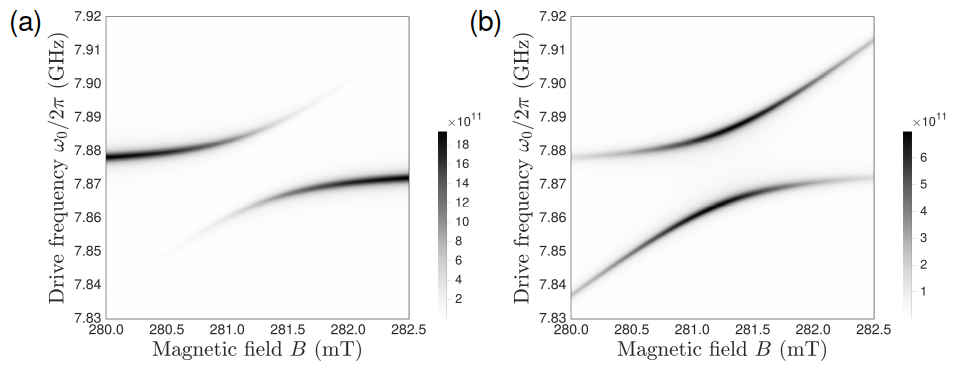
\includegraphics[width=2\basefigurewidth,clip]{./figure/4_1}
	\caption{强耦合参数下光子和磁振子平均粒子数的稳态谱} 
	\label{SC1stOrder}
\end{figure}
可以看到光子和磁振子平均粒子数的稳态谱中都出现了明显的反交错现象,并且光子的谱中围绕腔共振频率$\omega_c/2\pi$附近的强度最高,和实验上的特征一致,而磁振子谱则是围绕YIG球共振磁场附近的强度最高。

腔磁振子系统的稳态解\eqref{photon_num}以及\eqref{magnon_num}都可以看作是由两部分所构成,即相干部分$|\overline{\alpha_{0}}|^{2}$、$|\overline{\beta_{0}}|^{2}$以及由$\overline{n}_c$、$\overline{n}_m$决定的热部分。而在图\ref{SC1stOrder}的参数范围内可以计算出热占据数$\overline{n}_c\approx\overline{n}_m$在$793\pm5$小幅度变化,因此图\ref{SC1stOrder}的强度变化主要是由相干部分导致的。

对于稳态谱中的反交错现象可以这样理解,我们由孤立腔磁振子系统的哈密顿量
\begin{equation}
H_{iso} = \hbar\omega_{c}c^{\dag}c+\hbar\omega_{m}m^{\dag}m+\hbar gc^{\dag}m+\hbar gm^{\dag}c
\label{HamiltonianIsolated}
\end{equation}
可以将其变换为两个独立的polariton模式,并得到两个本征频率$\omega_p^{up}=\frac{1}{2}\Big[(\omega_c+\omega_m)+\sqrt{(\omega_c-\omega_m)^2+4g^2}\Big]$,$\omega_p^{down}=\frac{1}{2}\Big[(\omega_c+\omega_m)-\sqrt{(\omega_c-\omega_m)^2+4g^2}\Big]$。而在强耦合参数$g\gg\kappa_c,\kappa_m$下$\omega_p^{up}$,$\omega_p^{down}$正是\eqref{photon_num}与\eqref{magnon_num}关于驱动频率变量$\omega_0$的两个极大值点,因此不难理解当驱动频率调节到系统的本征频率附近时会出现共振并极大的增强系统中的光子和磁振子场。但是由于驱动场只输入相干光子,相干磁振子是通过耦合转化过来的,导致了图\ref{SC1stOrder}(a)和(b)中稳态谱强弱分布的差异。

有了能够和实验对比的光子和磁振子场的平均粒子数稳态谱后,我们接下来就有信心继续给出腔磁振子系统二阶关联函数的稳态谱。但是直接计算图\ref{SC1stOrder}所使用的实验参数下的二阶关联函数谱并不能得到很多信息,这点从\eqref{g2pho}和\eqref{g2mag}中就可以看出,因为此时的相干部分$|\overline{\alpha_{0}}|^{2},|\overline{\beta_{0}}|^{2} \gg n$,所以$g_{pho}^{(2)}(0)$和$g_{mag}^{(2)}(0)$在测量意义上等于1,也就是说此时的光子和磁振子都处于相干态。要想得到包含有用信息的二阶关联函数稳态谱,我们必须意识到目前的腔磁振子系统中存在着由外加驱动输入的相干部分以及由热环境导致的退相干部分的竞争,当某一部分过大时另一部分的要素就会被淹没在其中,这一点我们可以从图\ref{CoherentVary2edOrder}中看出。
\begin{figure}[htbp]
	\centering
	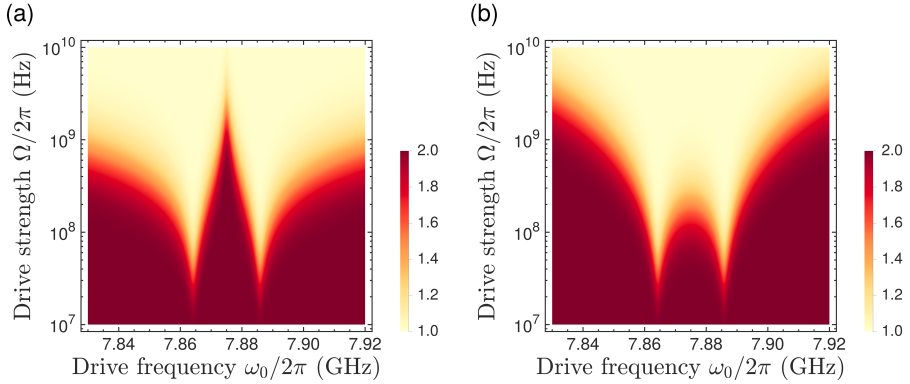
\includegraphics[width=2\basefigurewidth,clip]{./figure/4_2}
	\caption{光子和磁振子的二阶关联函数随驱动强度和驱动频率变化的二维颜色图} 
	\label{CoherentVary2edOrder}
\end{figure}
在图\ref{CoherentVary2edOrder}(a)和(b)中,我们分别绘制了当磁振子和腔中光子共振时二阶关联函数$g_{pho}^{(2)}(0)$和$g_{mag}^{(2)}(0)$在外加驱动强度$\Omega/2\pi$从$10^{10}$Hz减到$10^{7}$Hz的过程中随驱动频率$\omega_0/2\pi$变化的谱线,其他参数均和图\ref{SC1stOrder}一致。由于退相干部分保持不变,图\ref{CoherentVary2edOrder}实际上为我们展示了在相干部分“退潮”的过程中原本淹没在其中的退相干部分是如何逐渐显现出来的。当驱动强度过强时,$g_{pho}^{(2)}(0)=g_{mag}^{(2)}(0)=1$,系统中光子和磁振子都处于相干态,而当驱动强度过弱时,$g_{pho}^{(2)}(0)=g_{mag}^{(2)}(0)=2$,光子和磁振子又都处于热态。只有当相干部分和非相干部分竞争的不相上下时,二阶关联函数的稳态谱才会出现明显的强度分布。

\begin{figure}[htbp]
	\centering
	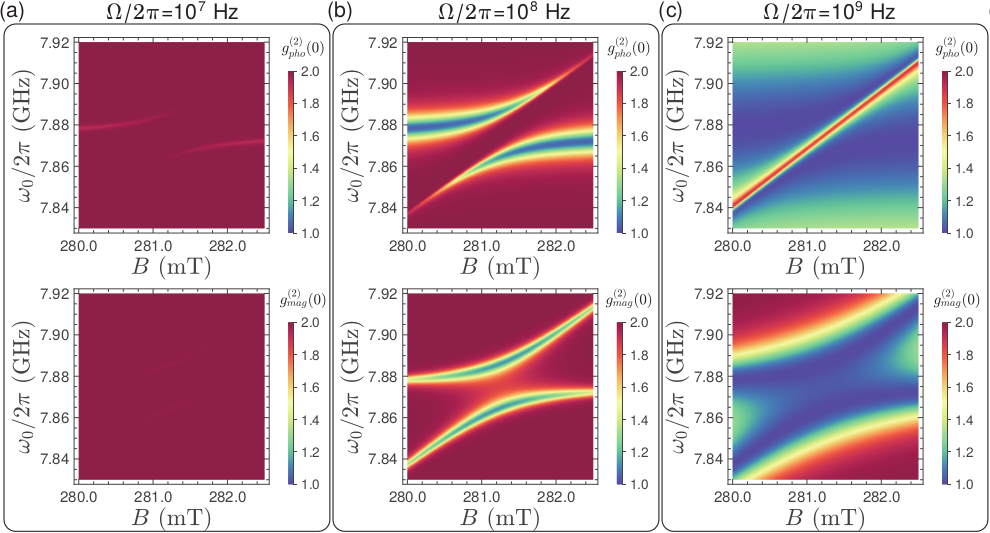
\includegraphics[width=3\basefigurewidth,clip]{./figure/4_3_1}
	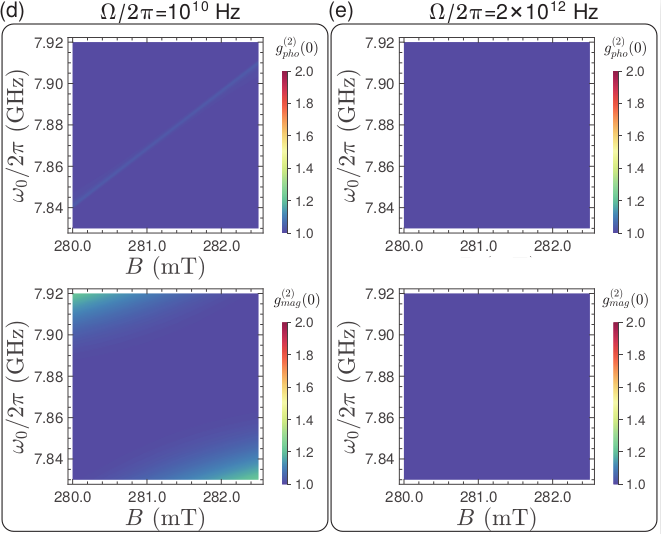
\includegraphics[width=2\basefigurewidth,clip]{./figure/4_3_2}
	\caption{不同驱动强度下的二阶关联函数稳态谱} 
	\label{Sepctrum2edOrder1}
\end{figure}
为了更直观和准确地理解腔磁振子系统中的相干竞争,我们可以像图\ref{SC1stOrder}一样计算二阶关联函数随外加驱动频率和偏置磁场变化的稳态谱。图\ref{Sepctrum2edOrder1}中我们展示了驱动强度$\Omega/2\pi$分别取$10^{7}$Hz,$10^{8}$Hz,$10^{9}$Hz,$10^{10}$Hz和$2$THz时具体的二阶关联函数稳态谱。其中当$\Omega/2\pi=10^{7}$Hz与$\Omega/2\pi=2$THz时,我们看到稳态谱都因为相干竞争的失衡而表现不出明显的变化。而在驱动强度增强的过程中,相干性增长最快的位置也处在polariton频率$\omega_p^{up}$和$\omega_p^{down}$上,图\ref{Sepctrum2edOrder1}(b)中二阶关联函数谱甚至表现出和平均粒子数谱一致的反交错现象。
\begin{figure}[htbp]
	\centering
	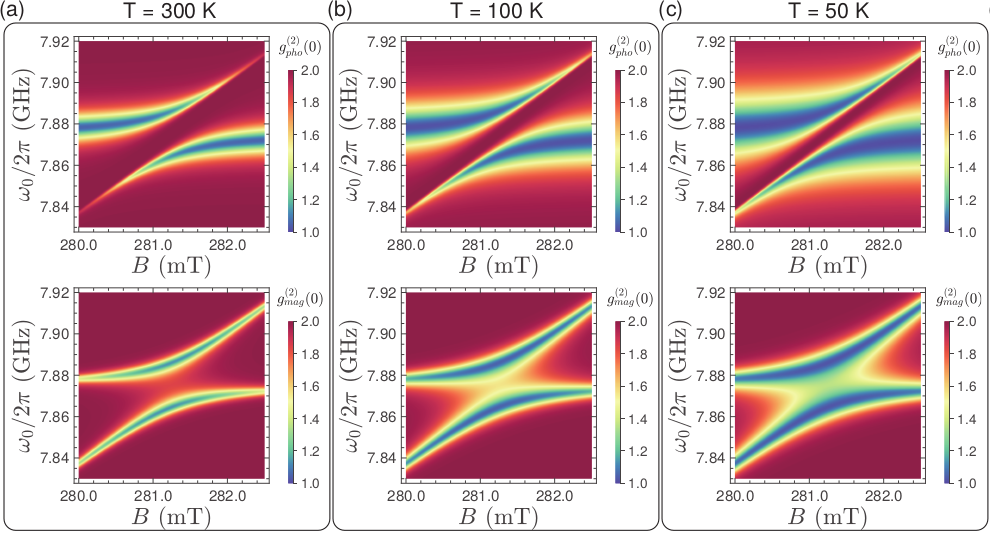
\includegraphics[width=3\basefigurewidth,clip]{./figure/4_4_1}
	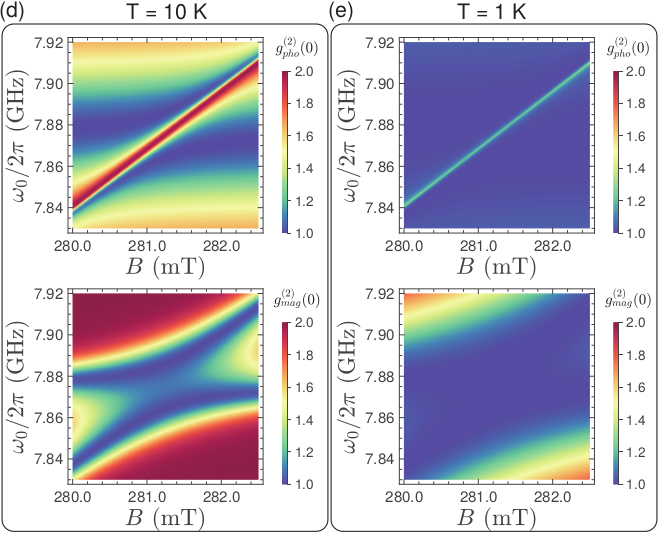
\includegraphics[width=2\basefigurewidth,clip]{./figure/4_4_2}
	\caption{不同温度下的二阶关联函数稳态谱} 
	\label{Sepctrum2edOrder2}
\end{figure}
在参数取定为图\ref{Sepctrum2edOrder1}(b)时,我们改变温度为$300$K,$100$K,$50$K,$10$K和$1$K,对应不同温度下的二阶关联函数稳态谱如图\ref{Sepctrum2edOrder2}(a)--(e)所示。可以看出,降低温度所引起的退相干部分减弱的效果与增强驱动的效果是一致的,当温度降低到退相干部分被完全压制的时候,腔磁振子系统就会表现为$g_{pho}^{(2)}(0)=g_{mag}^{(2)}(0)=1$的相干态。

\subsection{腔磁振子系统中的MIT现象}
由于腔磁振子系统的高度可调节性,Tang的实验中还实现了不同耦合参数下的测量。在耦合参数$\kappa_c>g>\kappa_m$时,系统中会出现MIT现象。MIT的称呼来源于以往的电磁诱导透明(EIT)现象,EIT指的是多能级原子和电磁场共振时,原本对探测电磁场的吸收会变为透明的现象,在实验中体现为测量谱线原本的洛伦兹线型会在峰值处出现一道尖锐的凹陷,腔磁振子系统中同样有着类似的实验现象。

我们选取参数为:$\omega_c/2\pi=\omega_m/2\pi=7.875$ GHz, $\kappa_m/2\pi=1.06$ MHz, $g/2\pi=10.8$ MHz, $\Omega/2\pi=1$ GHz 以及 $T=300$ K,绘制$\kappa_c/2\pi$增大的过程中光子和磁振子平均粒子数与二阶关联函数的稳态谱线如图\ref{MITkcVary}所示。
\begin{figure}[htbp]
	\centering
	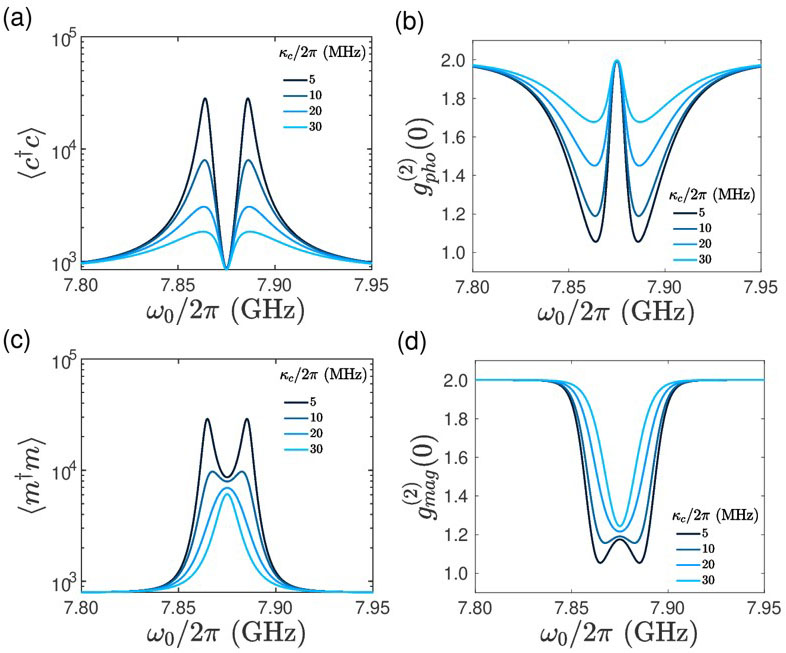
\includegraphics[width=2.1\basefigurewidth,clip]{./figure/4_5}
	\caption{微腔耗散率增大时光子和磁振子的稳态谱线} 
	\label{MITkcVary}
\end{figure}
可以看到,在单独增大微腔的耗散时,平均光子数一直保持着双峰的线型,但是两个对称峰的线宽一直在增大,峰值的位置依旧出现在$\omega_p^{up}$和$\omega_p^{down}$处。当$\kappa_c/2\pi=30$MHz时,耦合参数完全进入MIT区域,平均光子数的线型呈现极宽的线型中间出现一较窄线宽的凹陷,也就是经典EIT实验中的线型。在凹陷位置处$\omega_c=\omega_m=\omega_0$,由\eqref{first_order}可得光子相干部分$|\overline{\alpha_{0}}|^2 = \left(\frac{\Omega\kappa_{m}}{\kappa_{c}\kappa_{m}+g^{2}}\right)^2$保持十位数的量级,也就是说此处明明和其他位置处有着同样的耦合率、耗散率以及输入功率,与其他驱动频率处相比却几乎没有留住多少相干光子,造成这一结果的唯一原因在于稳态时的腔磁振子系统基本不再吸收输入光子,正是因为这样实验上此处的反射谱才会出现极大值,表示对输入光透明。尽管如此,我们只凭借平均光子数还是难以区分强耦合与MIT参数。但是在图\ref{MITkcVary}中我们发现平均磁振子数在两种参数下有着明显的不同,当$\kappa_c/2\pi$增大时平均磁振子数的谱线从双峰变为了单峰,这是由于在这种耗散占主导的参数下,耦合系统的本征频率不再有两个独立的解,因此我们可以结合磁振子谱线的行为来判断腔磁振子系统是否处于MIT现象的参数中。至于光子和磁振子的二阶关联函数,这里依旧存在着相干部分以及非相干部分之间的竞争,由公式\eqref{KcKmDefination}我们知道$\kappa_c$表征着系统与热环境的耦合强度,因此在$\kappa_c$增大时$g_{pho}^{(2)}(0)$和$g_{mag}^{(2)}(0)$都越来越接近于2,表明更接近于热态。

除了MIT现象的特征谱线之外,在$\kappa_c>g>\kappa_m$时,腔磁振子系统中还会出现法诺共振(Fano resonance)的线型。
\begin{figure}[htbp]
	\centering
	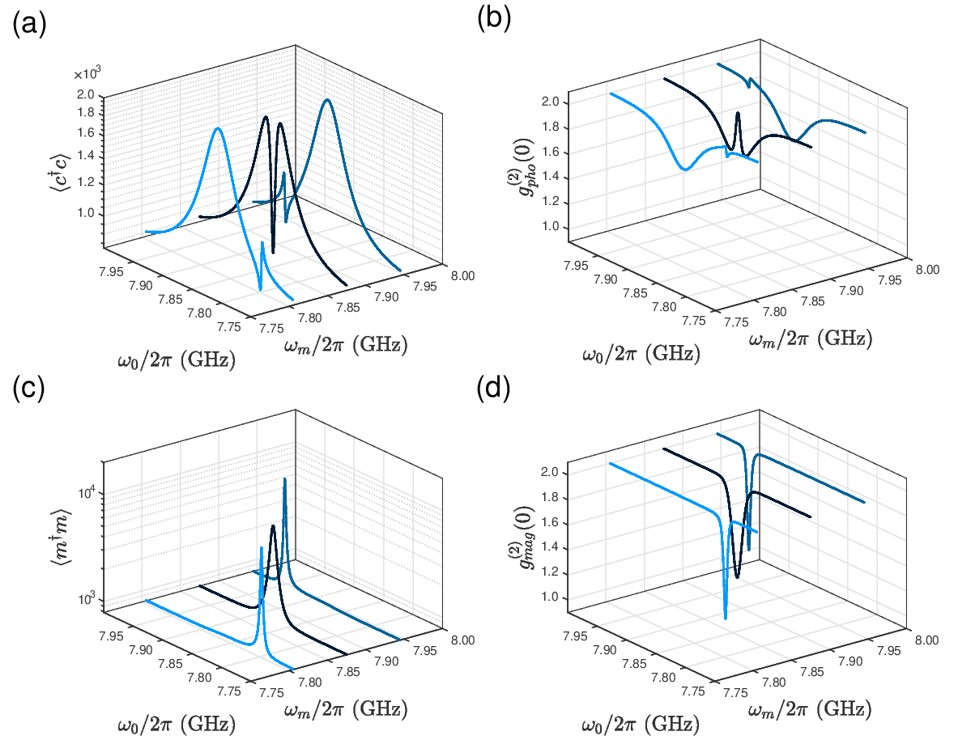
\includegraphics[width=2\basefigurewidth,clip]{./figure/4_6}
	\caption{MIT参数时不同磁场下光子和磁振子的稳态谱线} 
	\label{MITOmVary}
\end{figure}
如图\ref{MITOmVary}所示,我们在磁振子频率$\omega_m/2\pi$分别取7.805GHz,7.875GHz,7.945GHz时计算系统中平均粒子数与二阶关联函数的稳态谱线,其他参数为:$\omega_c/2\pi=7.875$ GHz, $\kappa_c/2\pi=30$ MHz, $\kappa_m/2\pi=1.06$ MHz, $g/2\pi=10.8$ MHz, $\Omega/2\pi=1$ GHz 以及 $T=300$ K。可以看到,在光子和磁振子的频率共振时,平均光子数的稳态谱线就是对称的MIT线型。而当二者远离共振的时候,本来出现在共振频率处的凹陷,我们称之为MIT窗口就会随着磁振子的频率而移动,并在磁振子频率附近出现了一个反对称的线型,也就是法诺线型。法诺共振广泛存在于有着背景和共振散射干涉的系统之中,通常使用法诺因子来表征这一非对称线型。我们这里的法诺因子可以由公式\eqref{first_order}导出,在远离共振的条件下$(\omega_c-\omega_0)\approx(\omega_c-\omega_m)$可以将光子的相干部分表示为
\begin{equation}
|\overline{\alpha_{0}}|^{2} =\frac{\Omega^{2}}{\kappa_{c}^{2}+(\omega_{c}-\omega_{m})^{2}}\frac{(q\Gamma+\omega_{0}-\omega_{1})^{2}}{\Gamma^{2}+(\omega_{0}-\omega_{1})^{2}}
\label{FanoEq}
\end{equation}
其中
\begin{gather}
\Gamma=\frac{g^{2}\kappa_{c}}{\kappa_{c}^{2}+(\omega_{c}-\omega_{m})^{2}} \\
\omega_{1}=\omega_{m}-\frac{g^{2}(\omega_{c}-\omega_{m})}{\kappa_{c}^{2}+(\omega_{c}-\omega_{m})^{2}}
\end{gather}
公式\eqref{FanoEq}中的参数 $q=(\omega_{m}-\omega_{c})/\kappa_c$ 即为法诺因子。从图\ref{MITOmVary}(a)中可以看出当法诺因子的正负性改变时,法诺线型的对称性也会跟着改变。在光子数的稳态谱表现出对称和非对称线型的时候,磁振子数的稳态谱一直保持着单峰并会随着偏置磁场改变位置,表现为铁磁共振的特征。

\subsection{腔磁振子系统中的Purcell效应}
\begin{figure}[htbp]
	\centering
	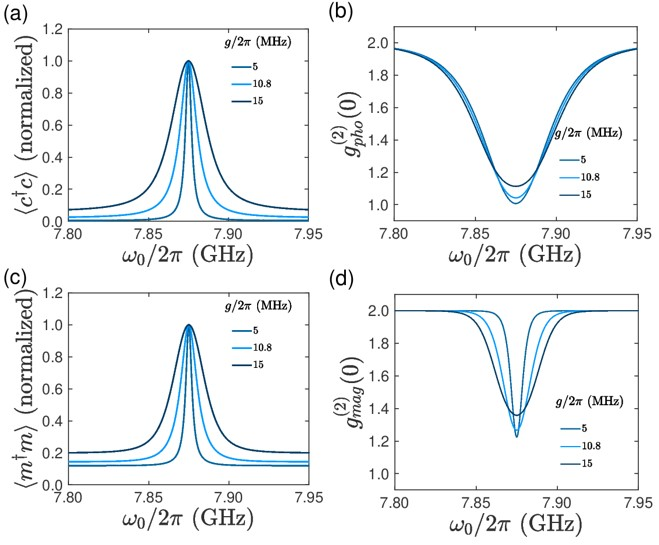
\includegraphics[width=1.9\basefigurewidth,clip]{./figure/4_8}
	\caption{腔磁振子系统中的Purcell效应} 
	\label{PurcellgVary}
\end{figure}
在Tang的实验中,当腔磁振子系统中耦合参数满足$\kappa_m>g>\kappa_c$时,测量结果还会表现出Purcell效应的特征。Purcell效应告诉我们光场与其他体系的耦合会引起光谱线宽的增强,这一增强的效果以一线型因子,即Purcell因子来表征。从图\ref{PurcellgVary}中我们可以直观看到Purcell增强的效应,当耦合率$g/2\pi$按照$5$MHz,$10.8$MHz,$15$MHz顺序增大时光子和磁振子的稳态谱线宽都会随之增宽,其中参数设置为:$\omega_c/2\pi=\omega_m/2\pi=7.875$ GHz, $\kappa_c/2\pi=1.35$ MHz, $\kappa_m/2\pi=30$ MHz, $\Omega/2\pi=1$ GHz 以及 $T=300$ K。而此时的Purcell因子同样可以由公式\eqref{first_order}导出,我们将一阶变量$\overline{\alpha_{0}}$整理为洛伦兹形式
\begin{equation}
\overline{\alpha_{0}}=\frac{\Omega}{i(\omega_{c}-\omega_{0})+\kappa_{c}\left(1+\frac{g^{2}}{\kappa_{c}\kappa_{m}}\frac{1}{1+\frac{i(\omega_{m}-\omega_{0})}{\kappa_{m}}}\right)}
\label{PurcellLine}
\end{equation}
当 $\kappa_m\gg(\omega_{m}-\omega_{0})$ 时,公式\eqref{PurcellLine}就变为了表示洛伦兹线型的公式,其洛伦兹线宽为 $\kappa_c(1+\frac{g^{2}}{\kappa_{c}\kappa_{m}})$。因此,我们说此时的光子数稳态谱在峰值附近处有着洛伦兹型的线型,而与磁振子的耦合导致了其洛伦兹线宽以Purcell因子$(1+\frac{g^{2}}{\kappa_{c}\kappa_{m}})$为倍数增强。

另一方面,我们还可以如图\ref{MITkcVary}一样,在改变磁振子的耗散率$\kappa_m$时观察稳态谱线是如何从强耦合转变为Purcell效应线型的。
\begin{figure}[htbp]
	\centering
	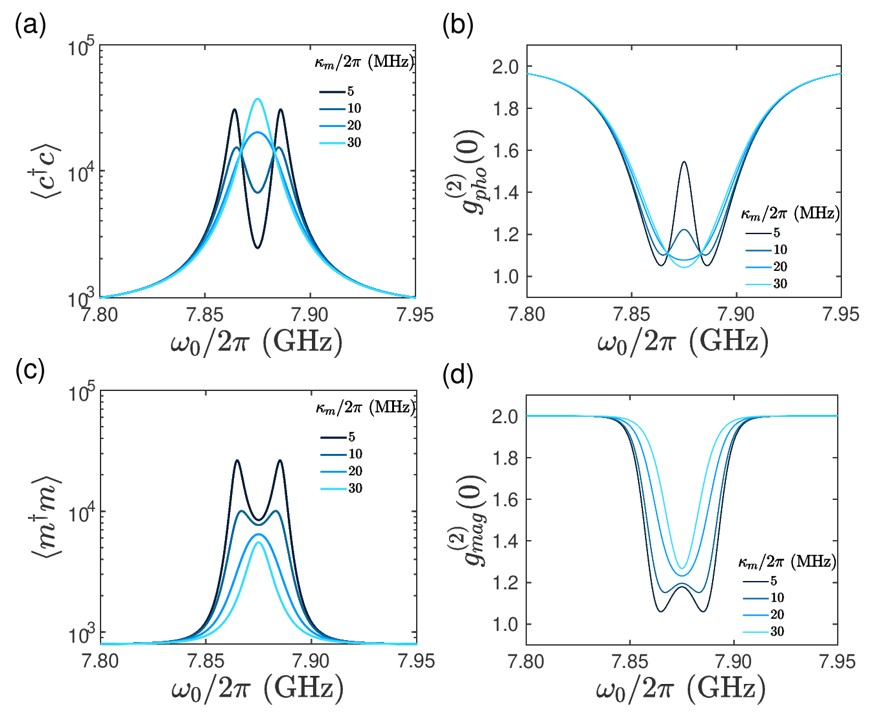
\includegraphics[width=1.9\basefigurewidth,clip]{./figure/4_7}
	\caption{磁振子耗散率增大时光子和磁振子的稳态谱线} 
	\label{PurcellKmVary}
\end{figure}
选取参数:$\omega_c/2\pi=\omega_m/2\pi=7.875$ GHz, $\kappa_c/2\pi=1.35$ MHz, $g/2\pi=10.8$ MHz, $\Omega/2\pi=1$ GHz 以及 $T=300$ K,计算$\kappa_m/2\pi$分别为$5$MHz,$10$MHz,$20$MHz,$30$MHz时的光子和磁振子稳态谱线如图\ref{PurcellKmVary}所示。在$\kappa_m/2\pi$增大的过程中,光子和磁振子稳态谱线都逐渐从双峰过渡为单峰。在$\kappa_m>g$之后,系统中的耦合地位逐渐降低,光子表现出解耦合的单峰线型,从Purcell因子可以看出,在$\kappa_m$增大到一定程度之后增强倍率会趋近于1。而磁振子耗散的增大使得稳态的相干磁振子数越来越少,$g_{mag}^{(2)}(0)$越来越趋近于2,磁振子也逐渐转变为热态。

% !TeX root = ../main.tex
% -*- coding: utf-8 -*-

\chapter{腔磁振子系统的动力学演化}
\label{ch5}

\section{相干部分演化的解析解}
在\ref{ch4}中我们了解到了存在于腔磁振子系统中的相干竞争,因此理解系统中相干部分的行为对于分析高阶量子关联而言是一种非常有效的途径。虽然我们没办法直接求解随机微分方程组\eqref{sdes1}--\eqref{sdes4},但是如果只关注一阶量的平均还是很容易继续处理的。

我们对方程组\eqref{sdes1}--\eqref{sdes4}中的随机变量取平均值,或者直接写出一阶量$\overline{\alpha}(t)$,$\overline{\beta}(t)$的级联方程\ref{HierarchicalEq}为
\begin{equation}
\begin{aligned}
d{\overline{\alpha}}&=(-i\omega_{c}\overline{\alpha}-ig\overline{\beta}+\Omega e^{-i\omega_{0}t}-\kappa_{c}\overline{\alpha})dt \\
d{\overline{\beta}}&=(-i\omega_{m}\overline{\beta}-ig\overline{\alpha}-\kappa_{m}\overline{\beta})dt 
\end{aligned}\label{Meansdes}
\end{equation}
方程组\eqref{Meansdes}是一组含时线性微分方程组,对于一定的初始条件可以使用拉普拉斯变换来求得方程组的特解。我们这里关注更特殊的一种情况,即在初始条件为$\overline{\alpha}(0)=\mathrm{c}_0$,$\overline{\beta}(t)=\mathrm{m}_0$,驱动强度$\Omega=0$时,方程组\eqref{Meansdes}的解满足
\begin{equation}
\left(\begin{array}{c}
\overline{\alpha}(t) \\
\overline{\beta}(t)
\end{array}\right)=\left(\begin{array}{c}
\mathrm{c} \\
\mathrm{m}
\end{array}\right) e^{-i \omega t}
\label{FormalSolution}
\end{equation}
而特征向量$(\mathrm{c} \quad \mathrm{m})^T$与特征频率$\omega$满足如下的本征方程
\begin{equation}
\left(\begin{array}{cc}
\omega_{c}-i \kappa_{c} & g \\
g & \omega_{m}-i \kappa_{m}
\end{array}\right)\left(\begin{array}{c}
\mathrm{c} \\
\mathrm{m}
\end{array}\right)=\omega\left(\begin{array}{l}
\mathrm{c} \\
\mathrm{m}
\end{array}\right)
\end{equation}
可以求得两个本征频率为
\begin{equation}
\omega_{\pm}=\frac{\omega_{c}+\omega_{m}}{2}-i \frac{\kappa_{c}+\kappa_{m}}{2} \pm \sqrt{\left(\frac{\omega_{c}-\omega_{m}}{2}-i \frac{\kappa_{c}-\kappa_{m}}{2}\right)^{2}+g^{2}}
\end{equation}
因此\eqref{FormalSolution}可以进一步表示为两个本征解的线性组合
\begin{equation}
\left(\begin{array}{c}
\overline{\alpha}(t) \\
\overline{\beta}(t)
\end{array}\right)=C_{+}\left(\begin{array}{c}
\mathrm{c}_{+} \\
\mathrm{m}_{+}
\end{array}\right) e^{-i \omega_{+} t}+C_{-}\left(\begin{array}{c}
\mathrm{c}_{-} \\
\mathrm{m}_{-}
\end{array}\right) e^{-i \omega_{-} t}
\end{equation}
这里的$\left(\mathrm{c}_{\pm} \quad \mathrm{m}_{\pm}\right)^T=\frac{1}{\sqrt{\left(\omega_{\pm}-\omega_{c}\right)^{2}+\kappa_{c}^{2}+g^{2}}}\left(g \quad \omega_{\pm}-\omega_{c}+i \kappa_{c}\right)^T$,系数$C_{\pm}$由初始条件定为$C_{\pm}=\frac{\pm \mathrm{m}_{\mp}\mathrm{c}_{0}}{\mathrm{c}_{+} \mathrm{m}_{-}-\mathrm{c}_{-} \mathrm{m}_{+}}$。

在强耦合参数下$g\gg\kappa_c,\kappa_m$,光子和磁振子的相干部分可以整理为如下形式
\begin{equation}
\begin{aligned}
|\overline{\alpha}(t)|^{2} &=\left|\mathrm{c}_{0}\right|^{2}(\mathcal{A}+\mathcal{B}+2 \mathcal{C} \cos (\Delta \omega t)) e^{-2 \kappa t} \\
|\overline{\beta}(t)|^{2} &=\left|\mathrm{c}_{0}\right|^{2} \mathcal{C}(2-2 \cos (\Delta \omega t)) e^{-2 \kappa t}
\end{aligned}\label{RabiOssilation}
\end{equation}
其中$\Delta \omega=\sqrt{\left(\omega_{c}-\omega_{m}\right)+4 g^{2}}$,and $\kappa=(\kappa_{c}+\kappa_{m})/2$,而三个系数$\mathcal{A}, \mathcal{B}, \mathcal{C}$ 为 $\mathcal{A}=$ $\frac{\left|\alpha_{+} \beta_{-}\right|^{2}}{\left|\alpha_{+} \beta_{-}-\alpha_{-} \beta_{+}\right|^{2}}, \mathcal{B}=\frac{\left|\alpha_{-} \beta_{+}\right|^{2}}{\left|\alpha_{+} \beta_{-}-\alpha_{-} \beta_{+}\right|^{2}}, \mathcal{C}=\frac{\left|\alpha_{+} \alpha_{-}\right|^{2}}{\left|\alpha_{+} \beta_{-}-\alpha_{-} \beta_{+}\right|^{2}}=$ $\frac{\left|\beta_{+} \beta_{-}\right|^{2}}{\left|\alpha_{+} \beta_{-}-\alpha_{-} \beta_{+}\right|^{2}}$。

\section{连续驱动下的动力学}
\begin{figure}[htbp]
	\centering
	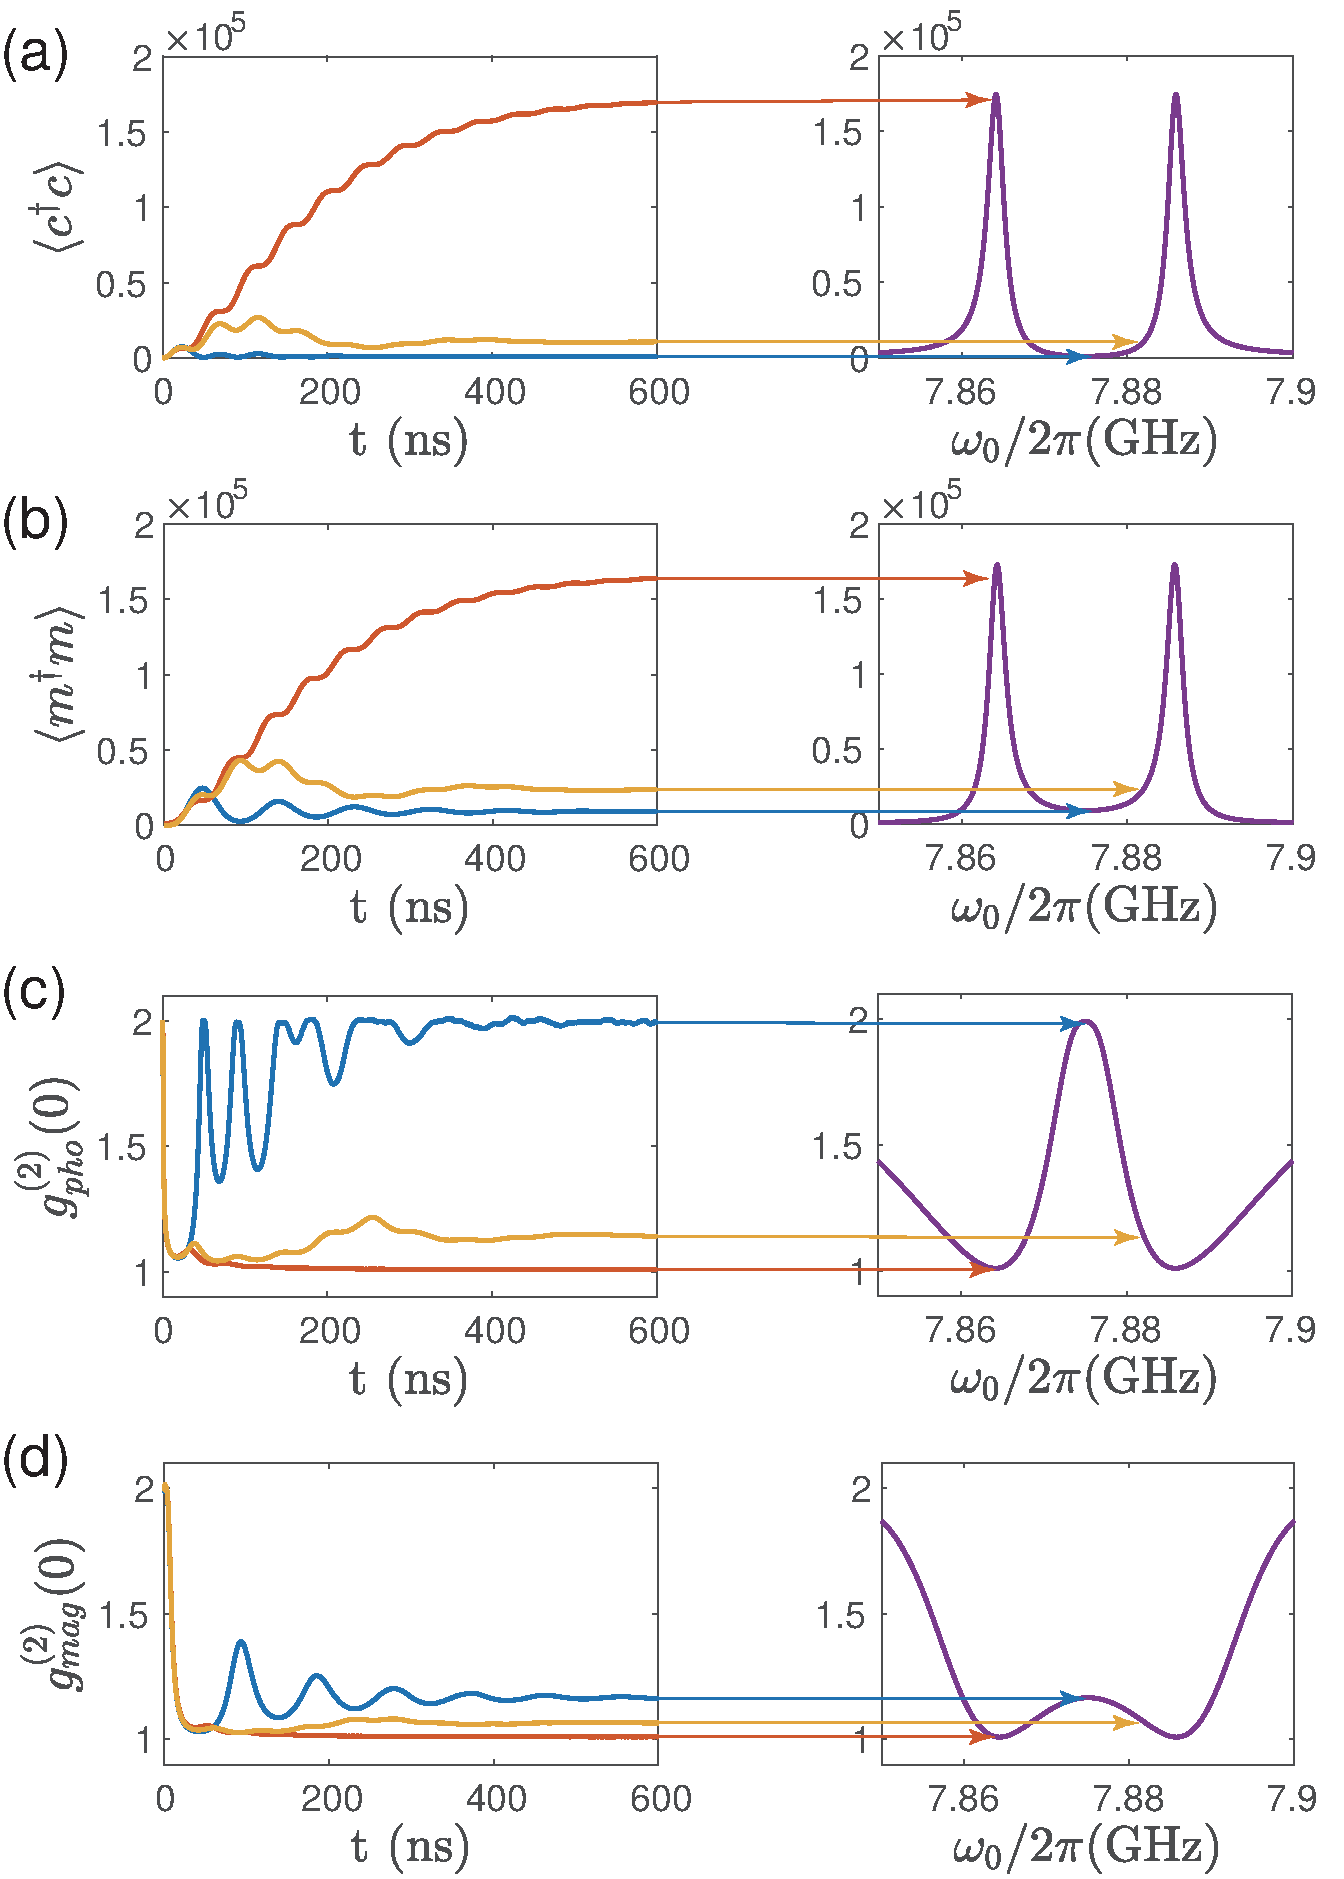
\includegraphics[width=1.7\basefigurewidth,clip]{./figure/5_1}
	\caption{连续驱动下系统由初态演化到稳态的过程} 
	\label{ContinuiousDrive2edOrder}
\end{figure}
这一节我们来演示怎样使用随机微分方程模拟的方法来得到系统在连续驱动下的动力学行为。在\ref{ch4}中我们得到了系统的稳态谱,但是对于腔磁振子系统如何在给定参数下从某一初始态演化为稳态的问题也是我们所感兴趣的。我们选取强耦合下的参数:$\omega_c/2\pi=\omega_m/2\pi=7.875$ GHz, $\kappa_c/2\pi=1.35$ MHz, $\kappa_m/2\pi=1.06$ MHz, $g/2\pi=10.8$ MHz, $\Omega/2\pi=1$ GHz 以及 $T=300$ K。设置初始时刻相干的光子数与磁振子数为0,随机微分方程算法的模拟步长为0.1ns,模拟样本的轨迹数量为100000。在图\ref{ContinuiousDrive2edOrder}(a)--(d)中我们模拟了600ns内$\omega_0/2\pi$取7.864GHz,7.875GHz,7.882GHz时系统中态的演化,并最终分别取平均计算了平均光子数$\langle c^{\dag}c\rangle$、平均磁振子数$\langle m^{\dag}m\rangle$以及二阶关联函数$g_{pho}^{(2)}(0)$、$g_{mag}^{(2)}(0)$。可以看到不同驱动频率下的光子和磁振子数都从0开始振荡着演化到了一个稳定值附近,而取更多个驱动频率后以稳定值和驱动频率的对应作图,我们就重新得到了腔磁振系统的稳态谱线。在收敛误差内,使用这一方法所得到的稳态谱线与\ref{ch4}中的结果是完全一致的,表明了我们的级联方程方法与随机微分方程模拟的方法在理论框架内是自恰的。

\section{脉冲激励后的时间演化}
连续驱动下的计算结果作为完善我们理论的一块拼图是十分有用的,但是目前的实验并不能对这种情况下的演化行为做出测量。在微波腔系统中,实验上通常是在使用一束持续时间极短的方波脉冲驱动激励腔体之后才能对腔中光场的瞬时动力学做出测量\cite{PhysRevLett.113.156401Tang,PhysRevB.99.134445Hu}。

为了和实验对照,我们选取参数:$\omega_c/2\pi=7.875$ GHz, $\kappa_c/2\pi=1.35$ MHz, $\kappa_m/2\pi=1.06$ MHz, $g/2\pi=10.8$ MHz, $\Omega/2\pi=0$, $T=300$ K。将模拟的初态相干光子数设置为$10^8$,相干磁振子数为0,抽样次数为100000,计算不同磁场下的平均光子数时间演化如图\ref{Evolution1stOrder}(a)所示。
\begin{figure}[htbp]
	\centering
	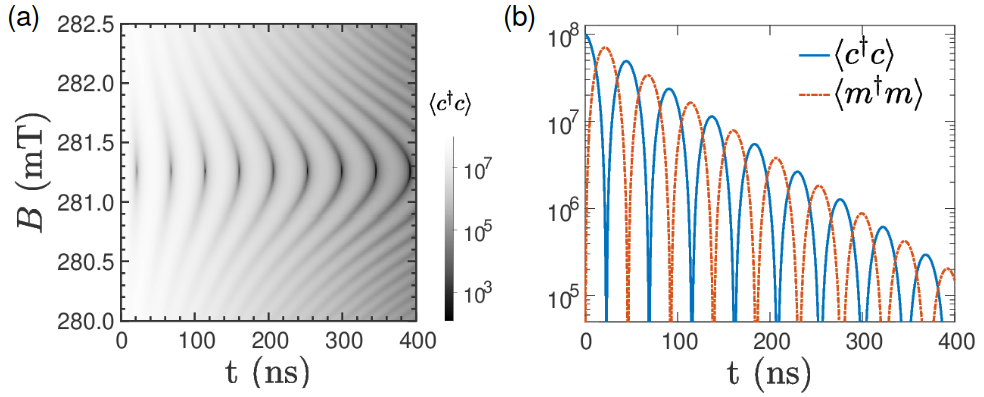
\includegraphics[width=2\basefigurewidth,clip]{./figure/5_2}
	\caption{脉冲激励后腔磁振子系统的Rabi振荡} 
	\label{Evolution1stOrder}
\end{figure}
可以看到在这种强耦合参数下,系统的瞬时动力学有着明显的振荡行为,并且随着时间的推进振荡的幅度也在一直衰减,而在磁场偏离共振的时候,由于耦合效率的降低,振荡行为也会减弱,这些特征都符合实验上的观测。为了更详细地观察系统中的振荡行为,我们取腔与磁振子共振时的磁场,把平均光子数和平均磁振子数的演化绘制在同一张图\ref{Evolution1stOrder}(b)上。我们看到腔与磁振子振荡的频率都和耦合率$g$相等,它们的相位相差$\pi$,并且振幅都随时间以相同速率指数衰减,这些行为都可以使用公式\eqref{RabiOssilation}来描述。实际上,这种表现出耦合率的振荡行为正是实现强耦合的标志之一,也就是腔QED中的Rabi振荡现象,我们这里的结果除了验证了对光场振荡行为的预测外,还证明了磁振子也有着同样的振荡行为。

虽然只靠相干部分就能理解腔磁振子系统中平均光子数和磁振子数中的Rabi振荡,但其实退相干部分的影响一直存在,我们可以从系统的二阶关联函数演化中更清晰的看到这一点。在图\ref{Evolution1stOrder}(a)的参数下,我们计算与其对应的二阶关联函数如图\ref{Evolution2edOrder}(a)所示,可以看到振荡行为此时在二阶关联函数中只出现在共振磁场的附近,偏离共振的位置处$g_{pho}^{(2)}(0)$和$g_{mag}^{(2)}(0)$都接近于1,光子和磁振子表现出极强的相干性。
\begin{figure}[htbp]
	\centering
	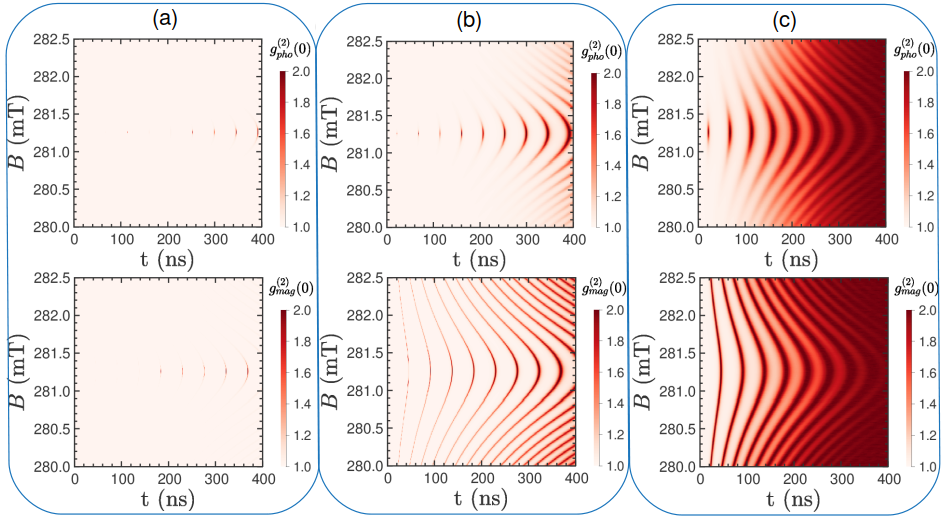
\includegraphics[width=3\basefigurewidth,clip]{./figure/5_3}
	\caption{不同初始激励下腔磁振子系统的二阶关联函数演化} 
	\label{Evolution2edOrder}
\end{figure}
与计算稳态谱时的做法类似,我们控制其他参量,依次调节初态激励的相干光子数为$10^8$,$10^6$,$10^4$,计算相应的二阶关联函数演化如图\ref{Evolution2edOrder}所示。我们同样可以看到在相干部分“退潮”的过程中,各个时刻下的非相干部分是如何显现出来的。对于相干部分与退相干部分竞争相当的图\ref{Evolution2edOrder}(b),我们再次观察到了和图\ref{Evolution1stOrder}(a)一样各处明显的振荡行为,只不过此时的振荡是光子和磁振子二阶关联函数的振荡,并且还在1与2之间变化,表明系统处于相干态和热态的频繁切换之中。另一方面,我们还可以控制温度的变化来调节非相干部分的影响。在图\ref{Evolution2edOrderTVary}中我们分别绘制了光子和磁振子共振时不同温度下系统的二阶关联函数演化,以方便更仔细地观察此时的Rabi振荡,在这里我们将初始相干光子数保持为$10^4$,其他参数和图\ref{Evolution2edOrder}(a)一致。
\begin{figure}[htbp]
	\centering
	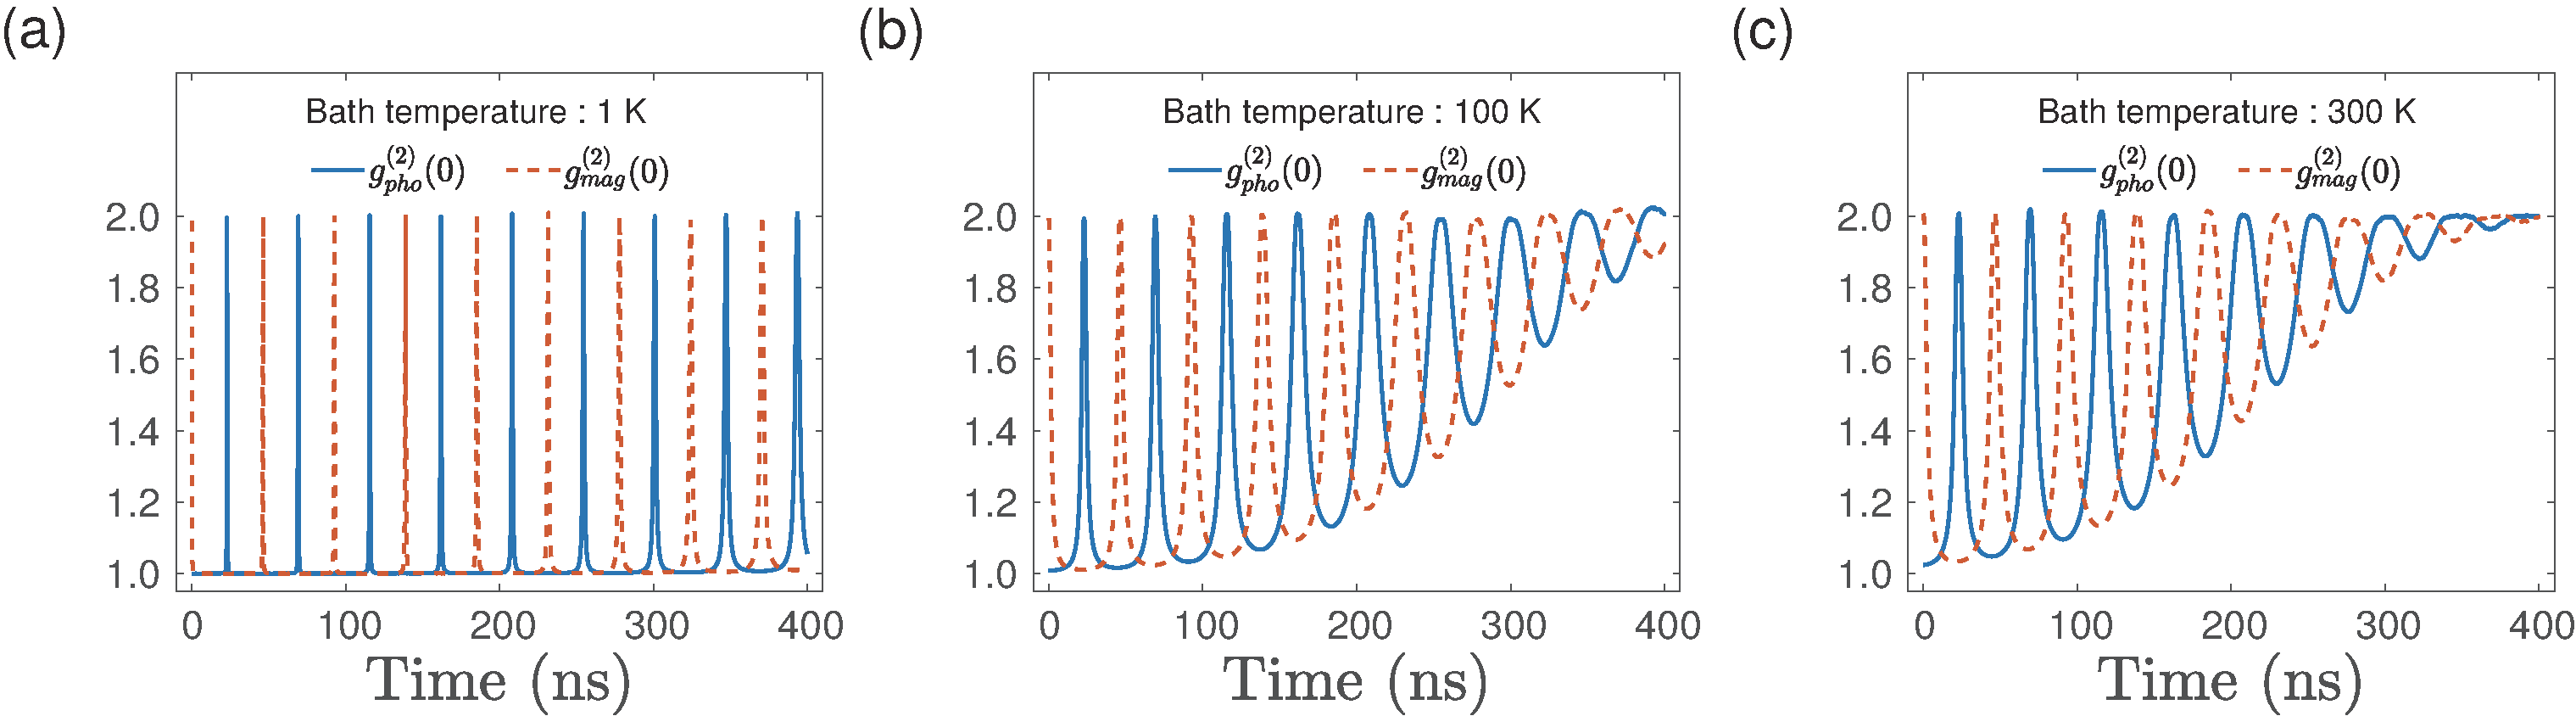
\includegraphics[width=3\basefigurewidth]{./figure/5_4}
	\caption{不同温度下腔磁振子系统的二阶关联函数演化} 
	\label{Evolution2edOrderTVary}
\end{figure}
我们可以看出,在温度升高的过程中退相干部分的增强使得各个时刻的二阶关联函数都更加趋向2,表示更快地趋向于热态。虽然此时的二阶关联振荡不再表现为三角函数曲线,但是振荡频率和相位依旧和相干部分的行为一致,说明是相干部分在主导振荡的行为。

\begin{figure}[htbp]
	\centering
	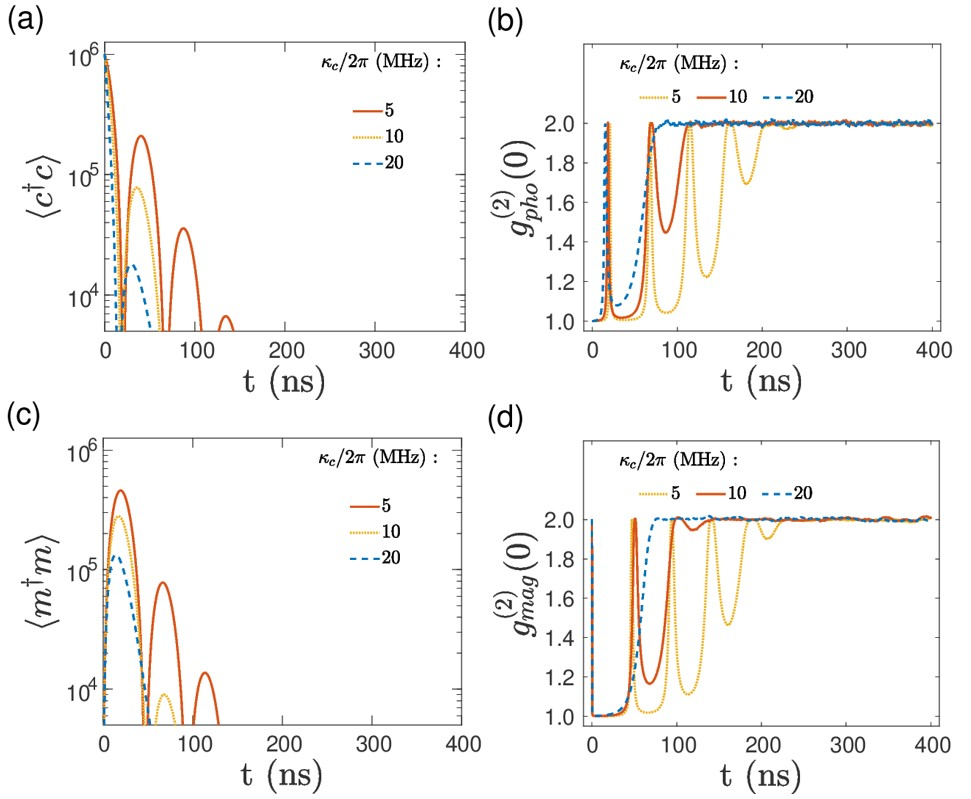
\includegraphics[width=2\basefigurewidth]{./figure/5_12}
	\caption{微腔耗散率增大时腔磁振子系统的时间演化} 
	\label{EvolutionMITKcVary}
\end{figure}
除了强耦合参数下脉冲激励后的时间演化,我们还探究了能出现MIT和Purcell效应参数下的情况。选取参数为:$\omega_c/2\pi=\omega_m/2\pi=7.875$ GHz, $\kappa_m/2\pi=1.06$ MHz, $g/2\pi=10.8$ MHz, $\Omega/2\pi=0$, $T=300$ K。在图\ref{EvolutionMITKcVary}中,我们依次取$\kappa_c/2\pi$为$5$MHz,$10$MHz,$20$MHz,计算出了对应情况下的平均粒子数以及二阶关联函数的演化行为。当$\kappa_c/2\pi=5$MHz,$10$MHz时,我们依旧能从光子和磁振子的演化曲线中看出Rabi振荡的痕迹,并且振荡的持续时间正比于$1/\kappa_c$。而当$\kappa_c/2\pi=20$MHz时,在这一耗散占主导的MIT参数下Rabi振荡的行为完全消失,初始激励的光子在很快的时间内因为耦合与耗散衰减为零,转化过来的相干磁振子又会通过耦合转换回光子,但是由于光子衰减的速率远大于磁振子的衰减速率,所以在磁振子衰减为零之后,相干光子已经全部耗散到环境之中了,最终系统中的光子和磁振子一起到达了热平衡的稳态。至于另外一个磁振子耗散占主导的情况,我们的做法类似,取$\kappa_c/2\pi=1.35$ MHz,保持其他参数和图\ref{EvolutionMITKcVary}一致,在$\kappa_m/2\pi$分别为$5$MHz,$10$MHz,$20$MHz时我们计算得到的系统演化行为如图\ref{EvolutionPurcellKmVary}所示。
\begin{figure}[htbp]
	\centering
	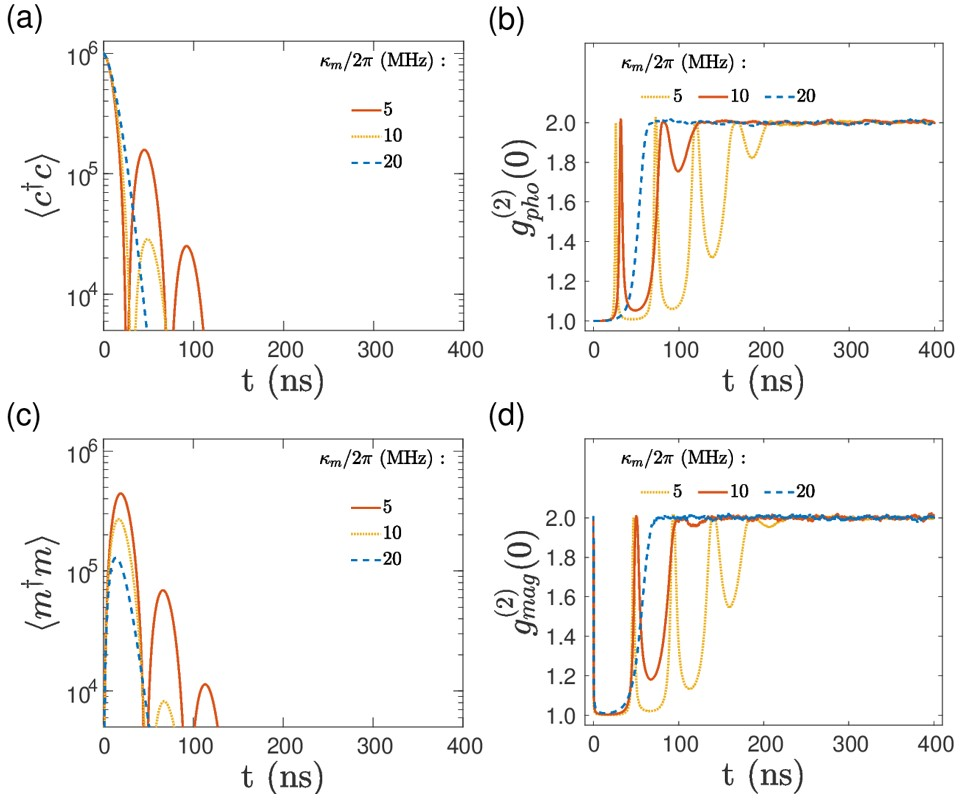
\includegraphics[width=2\basefigurewidth]{./figure/5_13}
	\caption{磁振子耗散率增大时腔磁振子系统的时间演化} 
	\label{EvolutionPurcellKmVary}
\end{figure}
同样地,我们可以看出在耗散尚未占据主导的时候,平均粒子数和二阶关联函数演化中的Rabi振荡持续时间正比于$1/\kappa_m$。而当$\kappa_m/2\pi=20$MHz时,在这Purcell效应的参数下Rabi振荡完全消失,同时由于磁振子衰减的速率反过来远大于光子的衰减速率,在磁振子获得相干能量之后就和光子一起衰减到了热稳态。在这个过程中,我们可以看出,由于与高耗散率YIG球的耦合,间接导致了光子衰减速率的增加,从\ref{EvolutionPurcellKmVary}(a)中我们可以明显看出光子的指数衰减速率要大于$\kappa_c/2\pi=1.35$ MHz,单看这一条衰减曲线就仿佛光子的耗散率增大了一样,这也正是Purcell效应在时间演化中的体现。


%%%%%%%%%%%%%%%%%%%%%%%%%%%%
% 论文其他信息
%%%%%%%%%%%%%%%%%%%%%%%%%%%%
% !TeX root = ../main.tex
% -*- coding: utf-8 -*-

\printbibliography[title=参考文献]

% !TeX root = ../main.tex
% -*- coding: utf-8 -*-

%\makeschapterhead{致谢}
\chapter*{致谢}
{
	\ttfamily \fontsize{12bp}{16bp}\selectfont
	感谢您使用本模板。
}
% !TeX root = ../main.tex
% -*- coding: utf-8 -*-

% !TeX root = ../main.tex
% -*- coding: utf-8 -*-

\chapter*{个人简历}


{
	\fontsize{10.5bp}{16bp}\selectfont
	赵国淦,出生于1997年11月20日。
	在2019年毕业于华东理工大学应用物理学专业并获得理学学士学位。
	于2019年至今在南开大学就读凝聚态物理研究生。
}


\section*{\leftline{研究生期间发表论文:}}
% 学术论文研究成果按发表的时间顺序列出
% (已发表的列在前面,已接收待发表的放在后面)
% 格式方便阅读为主可参考百度学术Google学术

\begin{itemize}
	\fontsize{10.5bp}{16bp}\selectfont
	\item Guogan Zhao, Yong Wang and X.-F. Qian. Driven dissipative quantum dynamics in a cavity magnon-polariton system [J]. Phys. Rev. B, 2021, 104 (13): 134423.
\end{itemize}




% 其他成果有可添加
% \section*{\leftline{研究生期间其它成果:}}
% % 研究成果可以是在学期间参加的研究项目、申请的专利或获奖等
% \begin{itemize}
% 	\item 
% \end{itemize}


\end{document}
